\appendix

\section{Resource Construction}
\label{app:data}

\subsection{Benchmark composition by source and track}

\begin{table}[htbp]
\centering
\begin{minipage}[t]{0.56\linewidth}\vspace{0pt}
\centering
% Row pitch raised so this table ends level with its side-by-side partner
% (the construction-funnel table, which has more rows); see appendix.tex.
{\tabstyle\renewcommand{\arraystretch}{1.94}\setlength{\tabcolsep}{1.5pt}
\begin{tabular*}{\linewidth}[t]{@{\extracolsep{\fill}}>{\raggedright\arraybackslash}p{0.95in}>{\raggedright\arraybackslash}p{0.5in} r rrrrr@{}}\toprule
\textbf{Source} & \textbf{Track} & $n$ & \textbf{NC} & \textbf{CI} & \textbf{CO} & \textbf{OI} & \textbf{MI}\\\midrule
QACC & web-retr. & 145 & 69 & 46 & 14 & 7 & 9\\
SituatedQA & web-retr. & 141 & 43 & 50 & 6 & 32 & 10\\
ConflictingQA & web-retr. & 137 & 8 & 53 & 73 & 1 & 2\\
TRUST-ALIGN & refusal & 128 & 57 & 45 & 13 & 13 & 0\\
FreshQA & web-retr. & 85 & 33 & 8 & 2 & 27 & 15\\
WikiRevision & curated & 78 & 0 & 0 & 0 & 78 & 0\\
HotpotQA & curated & 19 & 0 & 19 & 0 & 0 & 0\\
HealthContradict & curated & 2 & 1 & 0 & 1 & 0 & 0\\
Misinformation & curated & 1 & 0 & 0 & 0 & 0 & 1\\
\midrule
\textbf{Total} & & \textbf{736} & \textbf{211} & \textbf{221} & \textbf{109} & \textbf{158} & \textbf{37}\\
\bottomrule\end{tabular*}}

\end{minipage}%
\hspace{0.02\linewidth}%
\begin{minipage}[t]{0.42\linewidth}\vspace{0pt}
\centering
{\tabstyle\setlength{\tabcolsep}{3pt}
\begin{tabular}[t]{@{}>{\raggedright\arraybackslash}p{0.63\linewidth}r@{}}\toprule
\textbf{Stage} & \textbf{Records}\\\midrule
Raw candidate rows from four source pools & 20{,}330\\
$-$ normalised overlaps with the training question set & $-598$\\
$-$ duplicate normalised queries & $-8{,}891$\\
Unique usable candidates & 10{,}841\\
Source-balanced selection (seeded) & 2{,}000\\
Retained with exactly ten documents & 1{,}878 (93.9\%)\\
\quad underfilled, excluded & 122\\
Human first-pass reviewed (canonical cleaned corpus) & 1{,}221\\
Selected non-refusal set & 800\\
Consolidated preselection/review population & 1{,}454\\
Final answerable benchmark records & 608\\\bottomrule
\end{tabular}}
\end{minipage}
\dualcaption{table}{tab:tracks}{tab:funnel}%
{\textbf{Benchmark composition by source and construction track.} NC = No conflict, CI = Complementary information, CO = Conflicting opinions/research outcomes, OI = Conflict due to outdated information, MI = Conflict due to misinformation. Track~A is web-retrieved, Track~B is the held-out refusal pool, Track~C is curated conflict. The curated track is class-targeted: all 78 WikiRevision items are temporal-supersession cases, supplying 49\% of that class, and all 19 HotpotQA items are complementary-evidence cases}%
{Non-refusal construction funnel, counts as observed in the retained
artifacts.}
\end{table}

Table~\ref{tab:tracks} gives the full breakdown referenced in
\S\ref{sec:data}. The three tracks are structurally distinguishable, which is
why we report them separately rather than as one pool. Track~A records carry
live retrieval URLs across $1{,}431$ distinct domains and five documents each.
Track~B records use placeholder URLs inherited from the upstream refusal
resource and are uniformly five documents. Track~C records are internally
homogeneous by source: all 78 Wikipedia-revision items have exactly four
documents drawn from a single domain with revision-dated URLs and all 19
multi-hop items have exactly ten documents with no URLs.

\subsection{Retrieval funnel}

The non-refusal track proceeds through the following stages
(Table~\ref{tab:funnel}). Counts are as observed in the retained artifacts.

Retrieval requests twenty results per query and retains at most ten, with a
query-focused window selected by a TAS-B dense bi-encoder
\citep{hofstatter2021tasb}. The released records carry a deterministic
five-document view of those ten, sampled by a seeded rule that takes two from
the top five and three from the bottom five; this is why Table~\ref{tab:data}
reports a mean of $5.03$ documents per benchmark record rather than ten. The
reduction keeps the evidence set answerable while preventing the conflicting
documents from always occupying the highest-ranked positions, which would
otherwise let a model succeed by attending to rank alone.

Two discontinuities in this funnel have no retained per-record selector and we
report them as observed rather than reconstructing a rule. First, $1{,}878$
candidates were assigned for first-pass review but the canonical cleaned corpus
contains $1{,}221$ unique reviewed records. The remaining discontinuity is that the quality selection from
the $1{,}454$-record consolidated population down to the released benchmark is
described by a documented predicate, acceptance, reviewer confidence, retrieval
quality, evidence sufficiency, conflict clarity, query specificity, source
reliability, relevant-document count and gold-answer feasibility, but no
per-record script was retained. Relatedly, 105 of the 608 answerable benchmark
records appear in the consolidated review population only as consensus-completed
entries rather than as first-pass reviews. The refusal track reduces from a
200-record curated subset to the 128 released records without a documented
reduction rule, though a 128-record refusal-quality review stratum with complete
agreement is retained.

\subsection{Verification of the released files}

All statistics below are computed directly from the released JSONL rather than
from construction logs (Table~\ref{tab:relverif}; Figures~\ref{fig:datacomp}
and~\ref{fig:dataqual}).

\begin{table}[htbp]\centering\tabstyle
\begin{tabular*}{\linewidth}{@{\extracolsep{\fill}}lrr@{}}\toprule
\textbf{Property} & \textbf{Train} & \textbf{Benchmark}\\\midrule
Records & 943 & 736\\
Duplicate identifiers & 0 & 0\\
Identifier overlap (train/val $\cap$ benchmark) & \multicolumn{2}{c}{0}\\
Document/note identifier misalignments & 0 & 0\\
Canonical \texttt{d1..dN} ordering & 943/943 & 736/736\\
Key fact on every non-irrelevant note & 5{,}886/5{,}886 & 3{,}393/3{,}393\\
Irrelevant notes carrying a key fact & 0 & 0\\
Notes retaining an annotator vote tally & 6{,}642/6{,}642 & 3{,}701/3{,}701\\
Unique source domains & 2{,}633 & 1{,}431\\
Mean snippet length (words) & 231 & 222\\
Quote is an exact contiguous span & 82.6\% & 81.1\%\\
Quote is snippet-anchored (exact/ellipsis/partial) & 95.6\% & 95.9\%\\
\bottomrule\end{tabular*}
\caption{Verification of the released files, computed directly from the released
JSONL rather than from construction logs.}
\label{tab:relverif}
\end{table}

\paragraph{An independent validity check on the refusal track.} Refusal-required
examples are not merely \emph{labelled} insufficient, the document-level
adjudication, which was performed independently of the abstention label,
confirms it. Decisive \textit{supports} verdicts occur on $3.6\%$ of refusal-track
documents against $39.3\%$ elsewhere, an eleven-fold difference.

\begin{figure}[htbp]
\centering
\begin{minipage}[b]{2.534in}
\centering
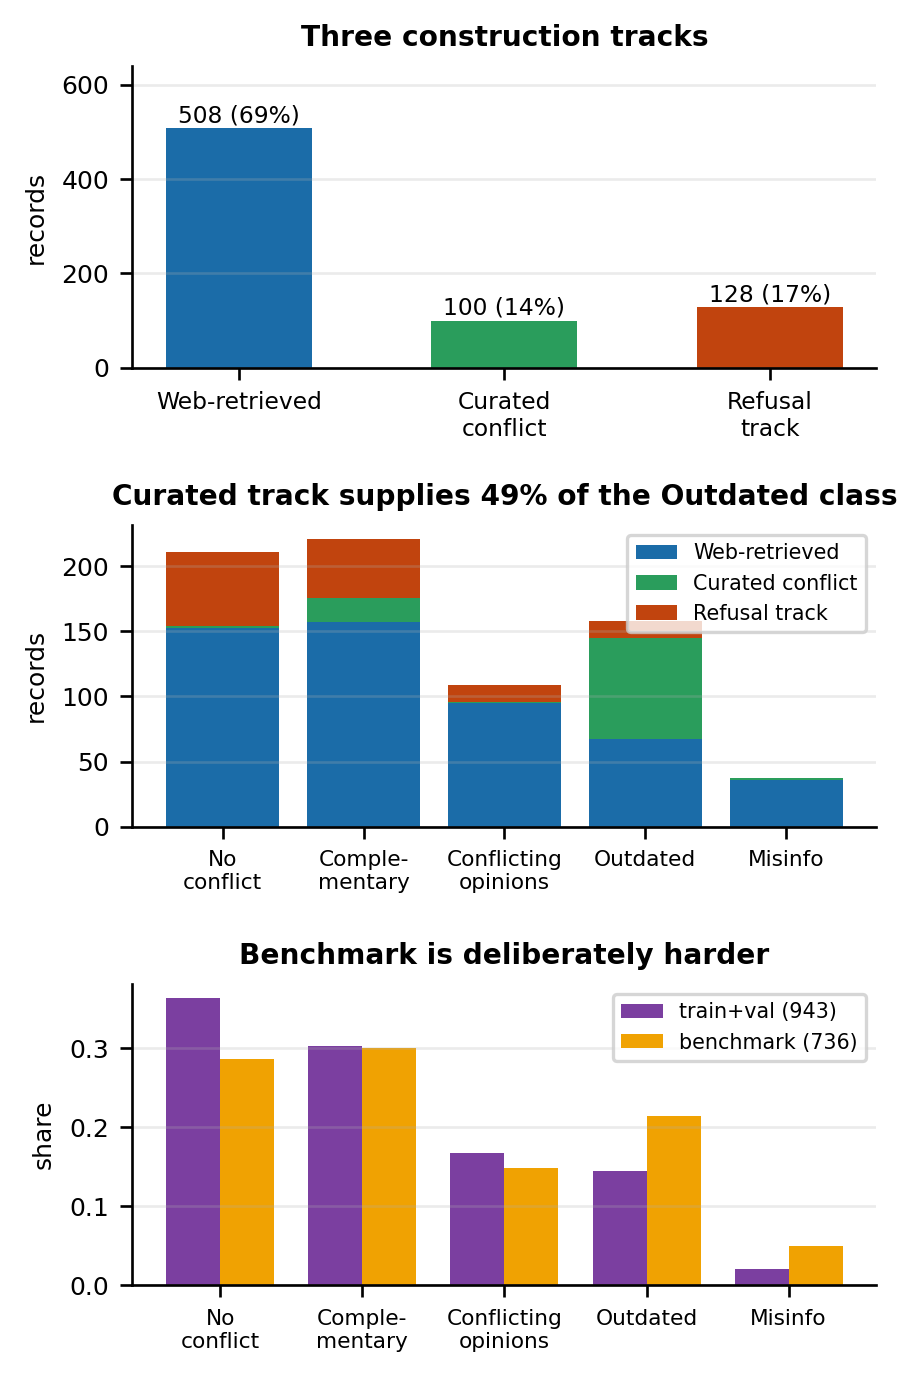
\includegraphics[height=3.785in]{figures/fig14_dataset_composition.png}
\end{minipage}
\hfill
\begin{minipage}[b]{2.766in}
\centering
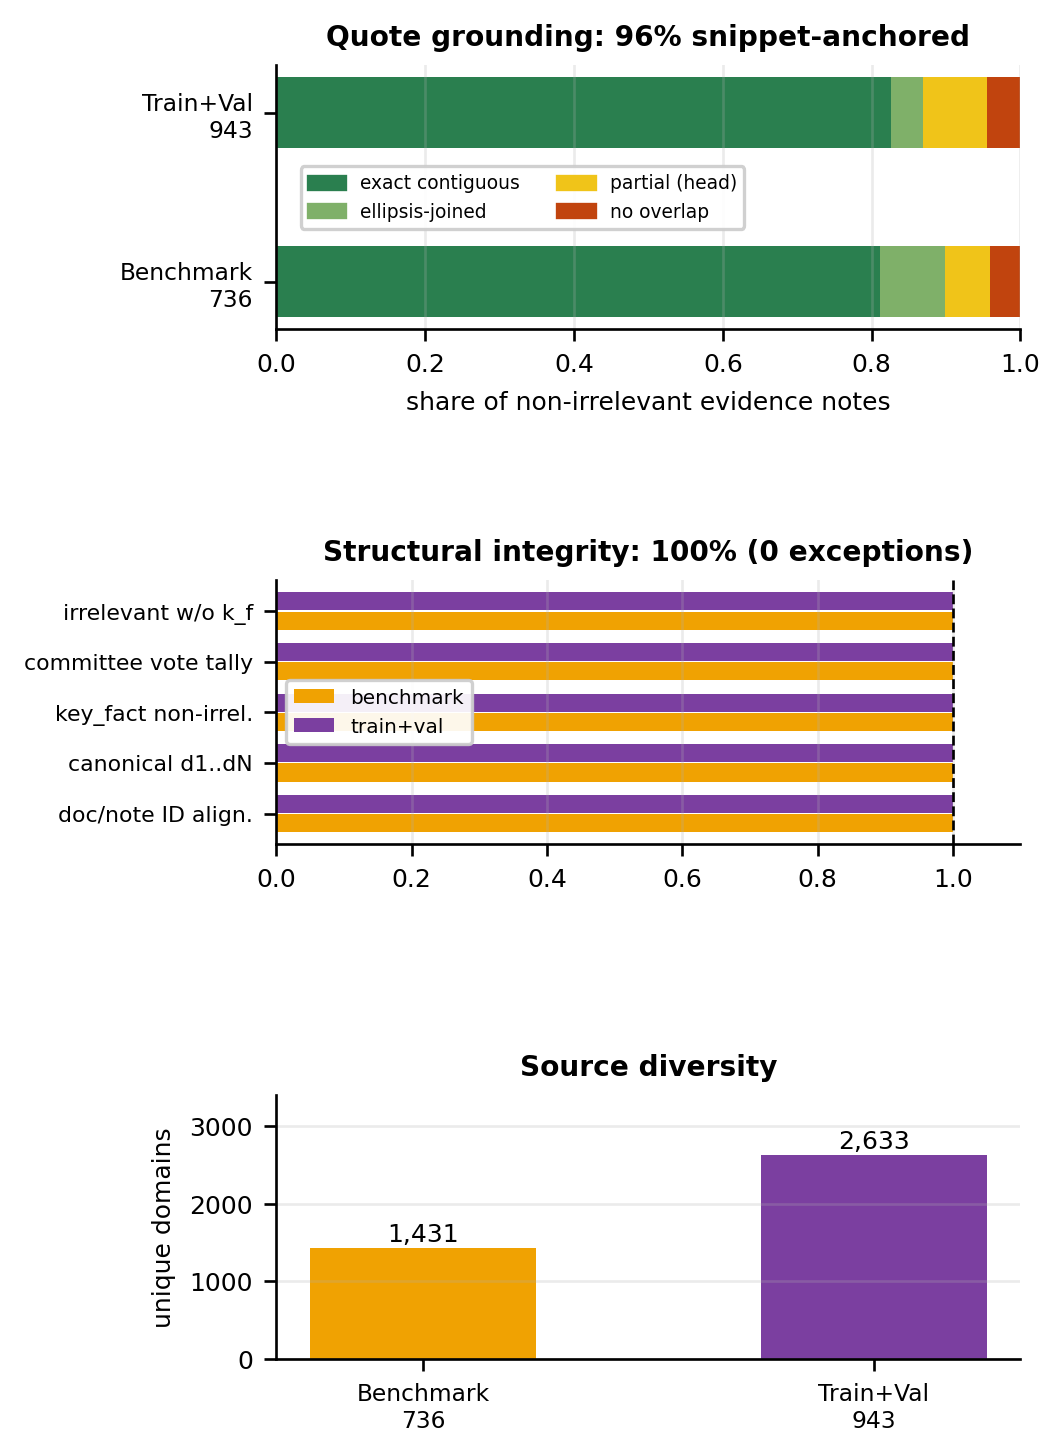
\includegraphics[height=3.785in]{figures/fig15_dataset_quality.png}
\end{minipage}
\dualcaption{figure}{fig:datacomp}{fig:dataqual}%
{Resource composition. Left: the three benchmark construction
tracks. Centre: the curated track is class-targeted, supplying $49\%$ of the
temporal-supersession class. Right: the benchmark is deliberately harder than
the training distribution, with fewer no-conflict and more
outdated/misinformation cases}%
{Quality audit computed directly from the released files.}
\end{figure}

\section{Annotation Pipeline}
\label{app:annotation}

Annotation is stagewise. At each stage every committee member independently
receives the same structured input and returns a structured output; the
committee votes only on the central categorical decision for that stage and
then adopts the associated natural-language explanation \emph{intact} from the
highest-weight member that supported the winning decision. The method therefore
combines committee agreement on decisions with a single internally coherent
reasoning bundle and never averages or splices prose from different annotators.

Formally, for a decision field with candidate values $v$, each successfully
represented annotator $m$ contributes its configured weight $w_m$ and the
system selects
\[
v^{*}=\arg\max_{v}\ \sum_{m} w_m\,\mathbf{1}[y_m=v],
\]
with exact ties broken deterministically by a fixed candidate ordering, so that
re-running the pipeline on identical inputs reproduces identical labels. Writing
$\mathcal{M}^{*}=\{m:y_m=v^{*}\}$ for the annotators on the winning side, the
explanation bundle is adopted \emph{intact} from
$m^{*}=\arg\max_{m\in\mathcal{M}^{*}} w_m$ rather than assembled field-by-field
across annotators, so a verdict, its quote and its rationale always originate
from one coherent interpretation. Every note retains
\texttt{\_vote\_tally}, \texttt{\_winner\_model} and \texttt{\_all\_verdicts},
so any label can be traced to its vote.

Stage-1 output is constrained: a verdict from the closed set, a key fact
anchored to a quoted span of at most 50 words, a verdict rationale and a
URL-derived source-quality label. The benchmark-mode Stage-1 prompt differs from
the ordinary prompt in one consequential way: older, contradictory or otherwise
conflict-bearing evidence about the target is retained as \textit{partially
supports} rather than discarded as \textit{irrelevant}, so that Stage~2 can see
the evidence needed to diagnose temporal and scientific conflicts at all.
Stage-2 votes the conflict label and the answerability flag; Stage-3 votes the
abstention decision independently of Stage-2 answerability, which is why a
complete analysis must inspect both fields.

Different retained artifacts were produced by different committee
configurations and we report the configuration alongside the artifact rather
than applying a single current default retrospectively. Structural validators
check schema conformance, label inventories and document/note alignment; they do
not establish quote entailment, factual correctness or temporal ordering, which
is why the human review of Appendix~\ref{app:human-review} is reported
separately rather than as a property of the automated pipeline.

\section{Human Review of the Resource}
\label{app:human-review}

Two workflows cover the two populations and must not be conflated. Both are
released with their raw per-reviewer files, assignment manifests, consolidated
pair records and machine-readable agreement metrics.

\subsection{Training conflict-type review}

All 658 base records were assigned to exactly two of three reviewers under a
seeded, pair-balanced, label-interleaved allocation, giving $1{,}316$ assignments
with loads of $439/439/438$ and reviewer-pair counts of $220/219/219$. Reviewers
saw the query, the retrieved snippets and the committee-assigned label, and could
retain it or replace it, recording confidence and a reason. This is a
label-validation protocol, not a keep/drop filter: no item is removed from the
pool by review.

\begin{table}[htbp]
\centering
\begin{minipage}[t]{0.47\linewidth}\vspace{0pt}
\centering
% Row pitch raised so this table ends level with its side-by-side partner
% (tab_benchiaa, which has more rows); see the pair in appendix.tex.
{\tabstyle\renewcommand{\arraystretch}{2.37}\setlength{\tabcolsep}{3pt}
\begin{tabular*}{\linewidth}[t]{@{\extracolsep{\fill}}l rr r@{}}\toprule
\textbf{Review field} & \textbf{agree} & \textbf{raw} & $\kappa$\\\midrule
Reviewed conflict type & 787 & 83.46\% & 0.7694\\
Retain-or-change action & 791 & 83.88\% & 0.1341\\
Changed-label (boolean) & 791 & 83.88\% & 0.1341\\
Reviewer confidence & 607 & 64.37\% & 0.0159\\
\bottomrule\end{tabular*}}

\end{minipage}%
\hspace{0.03\linewidth}%
\begin{minipage}[t]{0.47\linewidth}\vspace{0pt}
\centering
{\tabstyle\setlength{\tabcolsep}{2.5pt}
\begin{tabular*}{\linewidth}[t]{@{\extracolsep{\fill}}l rr r@{}}\toprule
\textbf{Review field} & \textbf{agree} & \textbf{raw} & $\kappa$\\\midrule
Preliminary conflict type & 1378 & 94.77\% & 0.9217\\
Retention decision & 1428 & 98.21\% & 0.9228\\
Retrieval quality & 1436 & 98.76\% & 0.9550\\
Evidence sufficiency & 1436 & 98.76\% & 0.9600\\
Conflict clarity & 1441 & 99.11\% & 0.9660\\
Query specificity & 1449 & 99.66\% & 0.9875\\
Source reliability & 1446 & 99.45\% & 0.9881\\
Relevant-document count & 1426 & 98.07\% & 0.9527\\
Gold-answer feasibility & 1440 & 99.04\% & 0.9669\\
Reviewer confidence & 1445 & 99.38\% & 0.9767\\
\bottomrule\end{tabular*}}

\end{minipage}
\dualcaption{table}{tab:trainiaa}{tab:benchiaa}%
{\textbf{Training conflict-type review agreement} over the 943-record consolidated population. The five-way taxonomy field is the primary result. The low chance-corrected values on the remaining rows reflect strongly imbalanced marginals (most reviewers accepted the committee label and reported high confidence), not label-quality failures: raw agreement and $\kappa$ answer different questions when one category dominates}%
{\textbf{Benchmark preselection agreement}, all ten recorded review fields over the $1{,}454$-record consolidated population. Every field exceeds $\kappa=0.92$. The primary result is the five-way conflict-type field. Because the second pass is sequential (Appendix~\ref{app:human-review}), these figures measure verification consistency rather than blind double annotation.}
\end{table}

The primary result in Table~\ref{tab:trainiaa} is the five-way conflict-type
field: $787$ of $943$ pairs agree, giving $83.46\%$ raw agreement and
$\kappa=0.7694$.

\paragraph{What the review layer actually changed.} Relative to the original
committee label, the first review retains it for $801/943$ records ($84.94\%$),
the second for $895/943$ ($94.91\%$), and both reviews retain it for $772/943$
($81.87\%$). The review layer is therefore doing real work: roughly one record in
five is contested by at least one reviewer.

\paragraph{Reviewer labels and released labels are different quantities.} The
consolidation deliberately does not overwrite the released \texttt{conflict\_type}.
The two distributions consequently differ, and we report both rather than
implying the review ratified the release. Reviewers' first-pass labels give
No conflict $373$, Complementary $289$, Outdated $130$, Conflicting opinions
$120$ and Misinformation $31$, against released counts of $343$, $286$, $136$,
$158$ and $20$. The largest divergences are the conflicting-opinions and
misinformation classes. Any analysis that treats the released label as
human-ratified would therefore overstate the evidence; we treat the review as a
reliability estimate on the taxonomy, not as a corrected gold standard.

\subsection{Benchmark preselection review}

Seven reviewers were allocated the $1{,}878$ exact-ten candidate set under seeded
source balancing, with non-uniform queues of $150/150/300/300/326/326/326$ and a
source mix of ConflictingQA $258$, FreshQA $394$, SituatedQA-temporal $413$,
QACC $407$ and SituatedQA-geographic $406$. Each reviewer recorded an acceptance
decision, a preliminary conflict type, confidence, retrieval quality, evidence
sufficiency, conflict clarity, query specificity, source reliability, a
relevant-document count bin, gold-answer feasibility and free-text notes.

Every one of the ten recorded fields in Table~\ref{tab:benchiaa} exceeds
$\kappa=0.92$, with the five-way conflict-type field at $94.77\%$ raw agreement
and $\kappa=0.9217$ ($1{,}378$ of $1{,}454$ pairs agreeing).

\paragraph{The second pass is sequential.} The second reviewer sees the complete
first review and may accept, edit or reject it; across the 800 selected records
there are $673$ accept-as-is and $127$ edited actions. These figures therefore
measure verification consistency and must not be presented as blind independent
double annotation. The second pass was nonetheless able to dissent: it introduced
label values the first pass never used, including $13$ \textit{Unsure}
conflict-type judgments and $15$ reject or borderline-reject retention decisions.

\paragraph{Reconstruction caveat.} Three second-review output files were lost and
were reconstructed after the corresponding reviewers confirmed that every first
review in their queue had been accepted as correct ($114$, $115$ and $114$
records). Those rows are therefore attested rather than independently recorded,
and the reconstruction manifest is released alongside the review data.

\subsection{Refusal-quality validation}
\label{app:refusalquality}

The $128$ released refusal items were reviewed as a separate stratum against four
dedicated fields in addition to the ten preselection fields. Agreement is
\emph{unanimous on all fourteen}: both reviewers judged all $128$ items to
require refusal, to have a valid abstention ground truth, to carry a
high-quality evidence-gap rationale, and to be a valid refusal benchmark item;
they also agreed unanimously that evidence is insufficient and that no defensible
gold answer is possible for any of them. Because each of these fields is
single-valued across the stratum, $\kappa$ is undefined and we report exact
agreement rather than substituting a coefficient.

This complements the automated check in Appendix~\ref{app:data}: decisive
\textit{supports} verdicts occur on $3.6\%$ of refusal-track documents against
$39.3\%$ elsewhere. The refusal targets are thus corroborated twice, once by
document-level adjudication performed independently of the abstention label and
once by unanimous human review.

\section{Fine-Tuning: Recipe Chronology}
\label{app:sft}

\subsection{Optimisation and checkpoint selection}

All models are fine-tuned with QLoRA
\citep{dettmers2023qloraefficientfinetuningquantized,hu2021loralowrankadaptationlarge}
at rank 32, $\alpha=64$ and dropout $0.05$, with learning rate
$2\times10^{-4}$, effective batch 16, maximum sequence length $12{,}288$ and
NEFTune $\alpha=5.0$ \citep{jain2023neftune}. Training minimises the standard
token-level cross-entropy of the serialised trace and final response given the
prompt and retrieved documents; no auxiliary loss term is added. Checkpoints are
selected on a held-out validation split by a composite score that sums
document-verdict accuracy, response-format validity and abstention correctness,
penalising false abstentions so that a model cannot score well by refusing
answerable questions. A \emph{recipe} is one fixed training mixture: the set and
proportion of task views and prompt variants a run is trained on. Qwen2.5-7B and
Qwen2.5-32B use recipe~K; Llama-3.1-8B and Mistral-7B use recipe~L.

The recipe was developed by error-directed revision rather than search.
Table~\ref{tab:recipe} names each intervention and its measured outcome,
including the two steps that did not work.

\begin{table}[htbp]\centering{\tabstyle
\begin{tabular*}{\textwidth}{@{\extracolsep{\fill}}llp{0.76\textwidth}@{}}\toprule
\textbf{Step} & \textbf{Rows} & \textbf{Intervention and outcome}\\\midrule
D & 6{,}699 & Strict/runtime/minimal multi-task mixture. \emph{Established that a trace survives minimal prompting.}\\
E & n/r & Broad conflict-label pressure. \textbf{Negative:} improved 32B conflict accuracy, degraded 7B. Capacity-sensitive.\\
F & 7{,}308 & One targeted taxonomy-boundary drill per source example. Best historical conflict result at both scales; narrower and more effective than E.\\
G & 8{,}526 / 8{,}715 & Model-specific probes: extra Stage-1 supervision (32B) and source-hygiene plus minimal-prompt pressure (7B). \textbf{Negative:} each recovered its target metric but cost conflict/contract quality.\\
J & 10{,}674 & \emph{Turning point.} Rebuilt train/validation geometry to include benchmark-like short answerable cases. Broad over-abstention substantially reduced; residual errors became localised.\\
K & 12{,}659 & +27 derived five-document answerable examples, document-boundary and partial-synthesis drills. Clean gain for 32B; genuine trade-off for 7B.\\
L & 13{,}349 & +21 short answerable \emph{no-conflict} examples, correcting a shortcut K risked introducing. Strong for Llama; Mistral still over-abstains.\\
\bottomrule\end{tabular*}}
\caption{\textbf{Fine-tuning recipe chronology.} Row counts are repeated supervised views, not independent questions. ``n/r'' marks a step whose exact mixture size was not retained.}
\label{tab:recipe}
\end{table}

Here ``n/r'' marks a step whose exact mixture size was not retained. Row counts
are repeated supervised \emph{views}, not independent questions:
recipe~L draws on 910 source examples. Three cautions apply to any causal
reading. J, K and L each change data coverage, drill composition and sample
weighting together, so they are principled recipe revisions rather than
single-factor ablations. The source-hygiene intervention explored at step~G is
\emph{not} present in the K/L mixtures and should not be attributed to the
reported models. And the reported matrices use recipe~K for the Qwen family and
recipe~L for Llama and Mistral, because no completed Qwen matrix exists for
recipe~L.

\section{Inference Protocol}
\label{app:inference}

Generation is deterministic at temperature $0$. Continuation budgets are
profile-specific, strict $1{,}400$ tokens base with a $3{,}200$ cap, runtime
$1{,}200/2{,}200$, minimal $900/1{,}800$, because a strict trace must enumerate
every retrieved document and a uniform cap would selectively truncate
long-context examples, confounding reasoning quality with output-space
availability. Generation halts on the sentinel.

A retry re-runs the \emph{identical} deterministic prompt with a larger token
budget when the structural contract is unmet. It never resamples, appends
corrective feedback, alters the retrieved documents or substitutes a prompt
profile. The minimal profile has no structural retry gate by default,
specifically to prevent the generation wrapper from turning a sparse-prompt
condition into a hidden strict condition.

Every run writes both a raw and a sanitised output file. Sanitisation may
canonicalise document order and identifiers, normalise label aliases, clear key
facts on irrelevant documents, drop out-of-range citations and append a missing
sentinel where a usable trace exists. It \emph{cannot} invent a missing trace,
construct absent document judgments, write a conflict analysis or supply a
missing answer; a record without a parseable trace passes through unchanged.

\section{CATS Specification}
\label{app:cats}

\subsection{Component definitions}

\paragraph{Grounded Refusal (GR).} Whether the system answered exactly when the
evidence permits answering. It is computed \emph{deterministically} from the
benchmark answerability label, never by a judge. We report refusal F1, where a
true positive is the model declining to answer when the retrieved evidence does
not support one.

\begin{table}[htbp]\centering{\footnotesize\renewcommand{\arraystretch}{1.15}\setlength{\tabcolsep}{3pt}
\begin{tabular}{@{}p{0.13\textwidth} p{0.34\textwidth} p{0.42\textwidth}@{}}\toprule
\textbf{Conflict type} & \textbf{Definition} & \textbf{Expected behaviour}\\\midrule
No conflict & All sources provide consistent and aligned information. & Return a unified, concise answer that synthesises the content accurately.\\
Complementary information & Sources provide different but non-contradictory pieces that complete each other. & Integrate all valid details into a richer, more comprehensive response.\\
Conflicting opinions or research outcomes & Sources disagree due to different viewpoints, experimental results or interpretations. & Present each viewpoint clearly, describe the nature of the disagreement, and avoid taking a side unless the evidence strongly supports one.\\
Outdated information & Some sources contain older data or conclusions that may no longer be reliable. & Prioritise newer, verified information while explicitly noting which sources are outdated.\\
Misinformation & A source provides factually incorrect, misleading or fabricated claims. & Reject or correct the misinformation, give the verified facts, and briefly explain why the claim is wrong.\\
\bottomrule\end{tabular}}
\caption{\textbf{The five conflict types}, their definitions and the response behaviour each requires. Stage~2 assigns exactly one label per example; Behaviour Adherence (\S\ref{sec:cats}) scores the response against the expected behaviour for the assigned type.}
\label{tab:taxonomy}\end{table}


\paragraph{Behaviour Adherence (BA).} Whether the answer followed the response
policy its conflict type requires, judged against a per-type rubric: a
no-conflict item expects a direct answer, complementary evidence expects
synthesis across documents, conflicting opinions expect both positions
represented without adjudication, outdated information expects the current value
with the superseded one flagged, and misinformation expects explicit correction.
The rubric is reproduced verbatim in Appendix~\ref{app:catsprompts}.

\paragraph{Factual Grounding (FG).} Whether each extracted claim is both
supported by an eligible retrieved document \emph{and} cited. Only documents
whose \emph{gold} per-document verdict is \textit{supports} or \textit{partially
supports} are eligible, so an answer that is true in the world but unsupported by
the retrieved set scores zero by construction. Support may be distributed across
a document pair.

\paragraph{Single-Truth Recall (STR).} Whether the response explicitly adopts the
target answer as its own conclusion, rather than merely quoting it, presenting it
as one of several possibilities, or attributing it to a source without endorsing
it. It is evaluated only for items where a single correct conclusion exists: no
conflict, complementary information, outdated information and misinformation
($n=487$). Conflicting-opinion items are excluded because no such conclusion
exists for them.

\subsection{Applicability and completeness}

For example $i$, let $A_i\in\{0,1\}$ be gold answerability, $\hat A_i$ the parsed
answer/refuse decision and $t_i\in\{1,\dots,5\}$ the conflict type. For a metric
$M$, write $\mathcal{I}_M$ for its applicable examples and $n_M=|\mathcal{I}_M|$.
Every dataset-level component below is an example-macro average over that set,
never an average over placeholder zeros. Correct refusals carry no
answer-content metrics, so
\[
\mathcal{I}_{\mathrm{BA}}=\mathcal{I}_{\mathrm{FG}}
=\{i:\neg(A_i=0 \wedge \hat A_i=0)\},
\]
\[
\mathcal{I}_{\mathrm{AQ}}=\mathcal{I}_{\mathrm{FG}},
\]
and $\mathcal{I}_{\mathrm{STR}}\subseteq\mathcal{I}_{\mathrm{FG}}$ additionally
requires a gold answer and a single-truth conflict type. An \emph{incorrect}
refusal remains in these denominators with zero extracted content; it is not
silently excluded. A headline aggregate is published only when every applicable
example has a score and every represented type has a value; otherwise the run is
marked incomplete rather than silently changing the denominator.

\subsection{Grounded Refusal}

The per-example decision gate is $g_i=\mathbf{1}[\hat A_i=A_i]$. With
``answered'' as the positive class,
\[
\mathrm{TP}=\textstyle\sum_i\mathbf{1}[\hat A_i{=}1,A_i{=}1],
\]
\[
\mathrm{FP}=\textstyle\sum_i\mathbf{1}[\hat A_i{=}1,A_i{=}0],
\]
\[
\mathrm{FN}=\textstyle\sum_i\mathbf{1}[\hat A_i{=}0,A_i{=}1],
\]
\[
\mathrm{TN}=\textstyle\sum_i\mathbf{1}[\hat A_i{=}0,A_i{=}0],
\]
giving $P_{\mathrm{ans}}=\mathrm{TP}/(\mathrm{TP}+\mathrm{FP})$,
$R_{\mathrm{ans}}=\mathrm{TP}/(\mathrm{TP}+\mathrm{FN})$ and
$F_{1,\mathrm{ans}}=2P_{\mathrm{ans}}R_{\mathrm{ans}}/(P_{\mathrm{ans}}+R_{\mathrm{ans}})$,
with a zero denominator yielding zero. The refusal-positive orientation swaps
$(\mathrm{TP},\mathrm{FP},\mathrm{FN},\mathrm{TN})\!\to\!(\mathrm{TN},\mathrm{FN},\mathrm{FP},\mathrm{TP})$:
\[
P_{\mathrm{ref}}=\frac{\mathrm{TN}}{\mathrm{TN}+\mathrm{FN}},\qquad
R_{\mathrm{ref}}=\frac{\mathrm{TN}}{\mathrm{TN}+\mathrm{FP}},
\]
and analogously $F_{1,\mathrm{ref}}$. Decision accuracy is
$(\mathrm{TP}+\mathrm{TN})/N$. Both orientations are reported because a model can
have near-perfect answer recall while refusing far too rarely, and because the
benchmark is $82.6\%$ answerable, so answering everything already yields
$608/736=0.826$ accuracy (\S\ref{sec:cats}).

\subsection{Committee voting rule for BA and STR}

The active local committee is Qwen3.5-397B-A17B, Mistral Small 4 and
DeepSeek-R1-Distill-32B with priorities $p_j=(6,3,2)$. On a binary judgment,
valid judge $j$ emits vote $z_{ij}\in\{0,1\}$ and confidence $c_{ij}\in[0,1]$,
contributing effective weight and vote masses
\[
a_{ij}=p_j\max(c_{ij},0.01),
\]
\[
W_i^{+}=\!\!\sum_{j:z_{ij}=1}\!\!a_{ij},\qquad
W_i^{-}=\!\!\sum_{j:z_{ij}=0}\!\!a_{ij}.
\]
The decision and the continuous positive support are
\[
d_i=\mathbf{1}[W_i^{+}>W_i^{-}],\qquad
u_i=\frac{W_i^{+}}{W_i^{+}+W_i^{-}}.
\]
A weighted tie is negative. Timeout, API and parse failures are removed before
forming these sums; an all-judge failure is recorded as an evaluation failure,
not interpreted as a confident negative.

\subsection{Behaviour Adherence}

Here $z_{ij}$ asks whether the response follows the type-specific behaviour
rubric (Appendix~\ref{app:catsprompts}). The reported component is binary,
\[
h_i=d_i,\qquad
\mathrm{BA}=\frac{1}{n_{\mathrm{BA}}}\sum_{i\in\mathcal{I}_{\mathrm{BA}}}h_i,
\]
whereas the aggregate uses the continuous support $b_i=u_i$. The distinction
preserves disagreement: a narrow weighted majority and a unanimous panel both
give $h_i=1$ but different $b_i$.

\subsection{Factual Grounding}

Let $\mathcal{D}_i^{+}$ be the documents whose gold per-document verdict is
\textit{supports} or \textit{partially supports}. The deterministic extractor
returns at most eight claims; for claim $k$, let $\mathcal{C}_{ik}$ be its
deduplicated cited-document set. FG uses \emph{raw priority} rather than
confidence, since its judge schema emits no per-document confidence. With
$\mathcal{J}_{ik}$ the valid judges,
\[
P_{ik}=\!\!\sum_{j\in\mathcal{J}_{ik}}\!\!\max(1,p_j),\qquad
\tau_{ik}=\frac{P_{ik}}{2},
\]
\[
m_{ik}=\begin{cases}2,&|\mathcal{J}_{ik}|>1,\\ 1,&|\mathcal{J}_{ik}|=1.\end{cases}
\]
For eligible document $d$, let $V_{ikd}=\sum_j\mathbf{1}[j\text{ names }d]$ and
$P_{ikd}=\sum_j\max(1,p_j)\mathbf{1}[j\text{ names }d]$. The accepted
claim-specific support set is
\[
\mathcal{S}_{ik}=\{d\in\mathcal{D}_i^{+} : P_{ikd}>\tau_{ik} \wedge V_{ikd}\geq m_{ik}\}.
\]
For cross-document support, let $x_{ikj}$ be judge $j$'s binary vote that two
documents jointly support the claim, with mass $X_{ik}=\sum_j\max(1,p_j)x_{ikj}$
and count $U_{ik}=\sum_j x_{ikj}$; the same thresholds give
$\chi_{ik}=\mathbf{1}[X_{ik}>\tau_{ik}\wedge U_{ik}\geq m_{ik}]$ and accepted
combination set $\mathcal{D}^{\times}_{ik}$. A claim earns credit only when
accepted support is \emph{actually cited}:
\[
y_{ik}=\mathbf{1}\big[(\mathcal{C}_{ik}\cap\mathcal{S}_{ik}\neq\emptyset)
\ \vee
\]
\[
(\chi_{ik}=1 \wedge \mathcal{C}_{ik}\cap\mathcal{D}^{\times}_{ik}\neq\emptyset)\big].
\]
For $K_i$ extracted claims,
\[
f_i=\begin{cases}K_i^{-1}\sum_{k=1}^{K_i}y_{ik},&K_i>0,\\ 0,&K_i=0,\end{cases}
\]
\[
\mathrm{FG}=\frac{1}{n_{\mathrm{FG}}}\sum_{i\in\mathcal{I}_{\mathrm{FG}}}f_i.
\]
The outer example-macro average prevents a long response from gaining weight
merely by yielding more claims. Under the full $(6,3,2)$ panel $\tau=5.5$: the
priority-6 judge clears the mass threshold alone but fails the two-judge
corroboration rule, while priorities $3+2$ fail the mass threshold, so no single
judge can unilaterally certify a document and the anchor judge must be joined by
at least one other (see Limitations).

\subsection{Single-Truth Recall}

STR applies when a gold answer exists and $t_i\in\{1,2,4,5\}$; type 3 is excluded
because conflicting-opinion cases need not have one canonical proposition. Let
$\mathcal{G}_i$ contain $M_i$ gold answer items. Applying the same weighted rule
to each item $\ell$, let $e_{i\ell}$ be the committee decision that the response
asserts that item as its own conclusion. For a negative decision the positive
side is the minority, so define a partial-credit indicator
\[
p_{i\ell}=\mathbf{1}\!\left[e_{i\ell}=0 \wedge
\frac{W_{i\ell}^{+}}{W_{i\ell}^{+}+W_{i\ell}^{-}}\geq 0.30\right],
\]
\[
E_i=\sum_{\ell}e_{i\ell},\qquad P_i=\sum_{\ell}p_{i\ell}.
\]
The per-example and dataset scores are
\[
r_i=\begin{cases}
0,& M_i=0\text{ or empty candidate},\\
1,& E_i>0,\\
\min\!\left(1,\tfrac{1}{2}\tfrac{P_i}{M_i}\right),& E_i=0,\ P_i>0,\\
0,&\text{otherwise},
\end{cases}
\]
\[
\mathrm{STR}=\frac{1}{n_{\mathrm{STR}}}\sum_{i\in\mathcal{I}_{\mathrm{STR}}}r_i.
\]
Quoting the gold item, listing it as one possibility among several, or
attributing it to a source without adopting it does not satisfy $e_{i\ell}=1$.

\subsection{Aggregation and its structural properties}
\label{app:aggregate}

The choice of aggregate is consequential: Figure~\ref{fig:aggchoice} shows that a
flat mean hides the refusal-calibration effect that both CATS aggregates surface,
and Figure~\ref{fig:refcredit} decomposes a headline score into the part earned
on answerable content and the part earned on the refusal decision alone.

\begin{figure}[htbp]
    \centering
    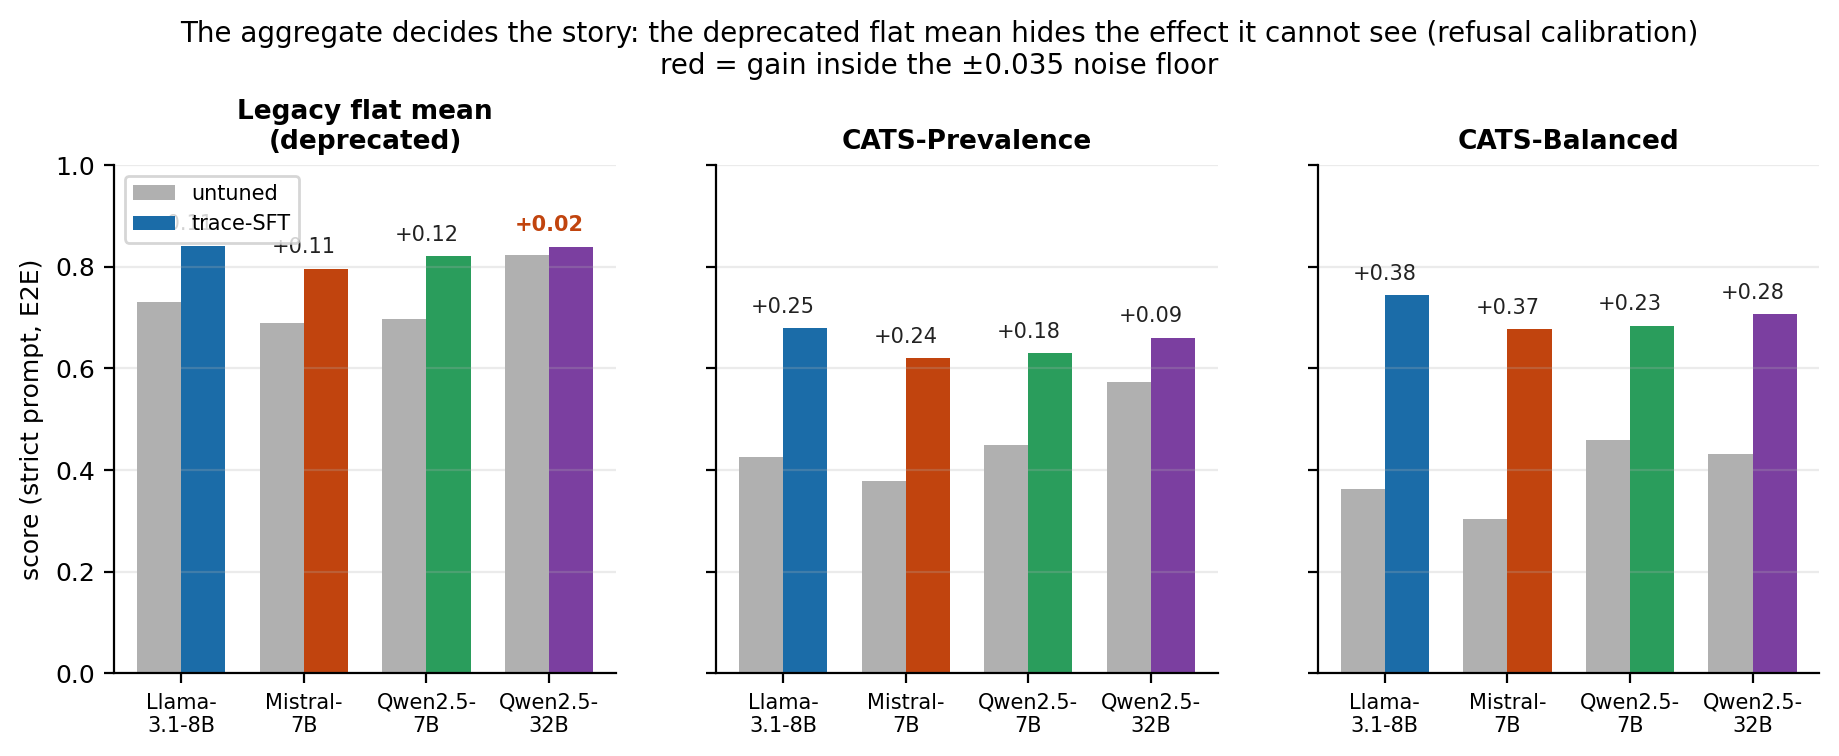
\includegraphics[width=0.95\textwidth]{figures/fig2_aggregate_choice.png}
    \caption{The choice of aggregate determines the conclusion. A flat mean over
    the four components hides the refusal-calibration effect almost entirely for
    Qwen2.5-32B, while CATS-Prevalence and CATS-Balanced both surface it. This is
    why we report components rather than a single number.}
    \label{fig:aggchoice}
\end{figure}

\begin{figure}[htbp]
    \centering
    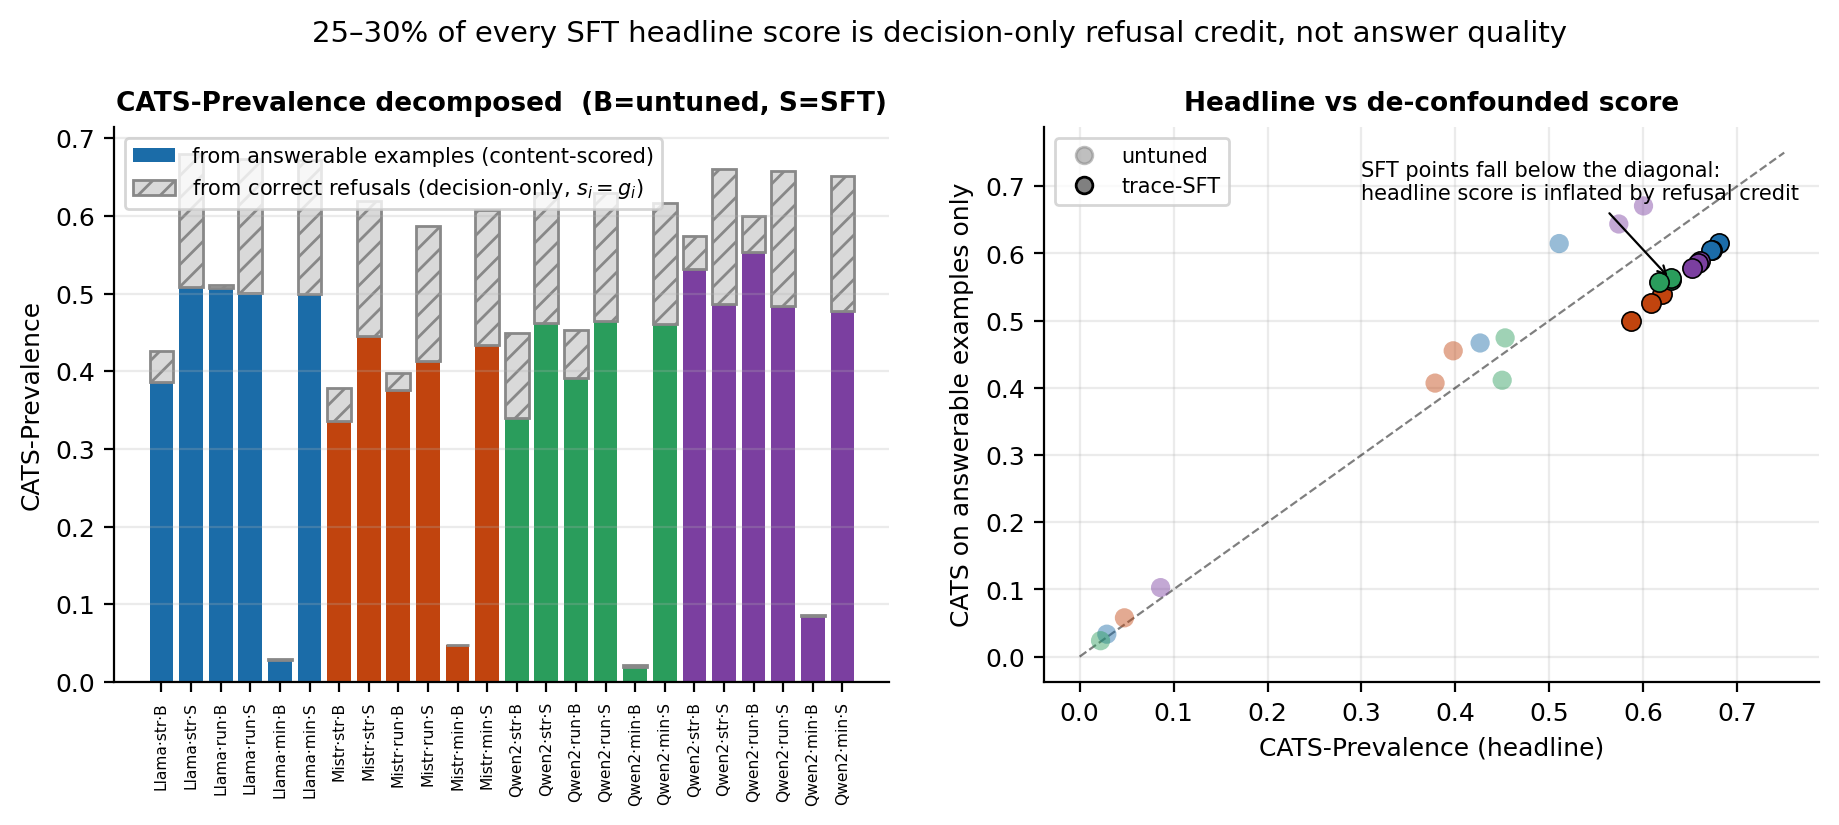
\includegraphics[width=0.95\textwidth]{figures/fig3_refusal_credit.png}
    \caption{Refusal credit inside the aggregate. Left: CATS-Prevalence split
    into the part earned on answerable examples and the part earned on correct
    refusals, which are scored on their decision alone. Right: plotting the
    answerable-only score against the headline places every trace-tuned point
    below the diagonal, showing the headline is inflated by decision credit.}
    \label{fig:refcredit}
\end{figure}


The three-step construction is as follows. Grounding and recall are averaged
\emph{geometrically} into an answer-quality term; that term is averaged
\emph{harmonically} with behaviour adherence; and the result is multiplied by the
grounded-refusal decision, which is $1$ when the answer/refuse choice was correct
and $0$ otherwise. Both means are used because they penalise imbalance: a high
score on one component cannot compensate for a low score on another, and a wrong
decision sets the example to zero regardless of everything else. CATS-Prevalence
is the plain mean over the benchmark; CATS-Balanced weights each conflict type
equally.

Per example, grounding and recall first form the answer-quality pillar
\[
q_i=\begin{cases}
\sqrt{f_i r_i},& i\in\mathcal{I}_{\mathrm{FG}}\cap\mathcal{I}_{\mathrm{STR}},\\
f_i,& i\in\mathcal{I}_{\mathrm{FG}}\setminus\mathcal{I}_{\mathrm{STR}},\\
\text{N/A},& i\notin\mathcal{I}_{\mathrm{FG}},
\end{cases}
\]
\[
\mathrm{AQ}=\frac{1}{n_{\mathrm{AQ}}}\sum_{i\in\mathcal{I}_{\mathrm{AQ}}}q_i.
\]
Let $H(x,y)=2xy/(x+y)$ for $x,y>0$ and $H(x,y)=0$ otherwise. The complete
per-example score is
\[
s_i=\begin{cases}
g_i,& A_i=0,\\
g_i\,H(b_i,q_i),& A_i=1,\ b_i,q_i\text{ available},\\
g_i b_i,& A_i=1,\ b_i\text{ only},\\
g_i q_i,& A_i=1,\ q_i\text{ only},\\
g_i,& A_i=1,\text{ neither available}.
\end{cases}
\]
The last three are auditable compatibility branches; complete benchmark runs use
only the first two. The decision gate means a wrong answer/refuse decision cannot
be rescued downstream, and the harmonic fusion penalises an answer that is weak
on either behaviour or answer quality rather than letting a strong one mask it.

To define the two headline summaries, let
$\mathcal{I}^{A}_t=\{i:t_i=t,A_i=1\}$ and $\mathcal{I}^{R}_t=\{i:t_i=t,A_i=0\}$,
with subgroup means
\[
T^{A}_t=\frac{1}{|\mathcal{I}^{A}_t|}\sum_{i\in\mathcal{I}^{A}_t}s_i,
\qquad
T^{R}_t=\frac{1}{|\mathcal{I}^{R}_t|}\sum_{i\in\mathcal{I}^{R}_t}s_i.
\]
The decision-balanced score for type $t$ is
\[
T^{\mathrm{DB}}_t=\begin{cases}
\tfrac{1}{2}(T^{A}_t+T^{R}_t),& |\mathcal{I}^{A}_t|>0,\ |\mathcal{I}^{R}_t|>0,\\
T^{A}_t,& |\mathcal{I}^{A}_t|>0,\ |\mathcal{I}^{R}_t|=0,\\
T^{R}_t,& |\mathcal{I}^{A}_t|=0,\ |\mathcal{I}^{R}_t|>0,
\end{cases}
\]
and the two reported aggregates are
\[
\boxed{\ \mathrm{CATS\text{-}P}=\frac{1}{N}\sum_{i=1}^{N}s_i\ }
\]
\[
\boxed{\ \mathrm{CATS\text{-}B}=\frac{1}{5}\sum_{t=1}^{5}T^{\mathrm{DB}}_t\ }
\]
CATS-P preserves benchmark prevalence. CATS-B gives each conflict type equal
weight and, within each type where both decisions occur, gives the answerable and
refusal-required subgroups equal weight. Both are secondary to the four
components (\S\ref{sec:cats}).

We disclose three consequences.

\paragraph{Refusal-required examples score decision correctness only.} Two
correct refusals receive the same score regardless of how well either is
justified. This is a scope choice, not an oversight: no consistently audited
refusal-quality judgment exists across the runs.

\paragraph{The type-balanced aggregate over-weights that decision.} Balancing
answerable and refusal subgroups within each conflict type gives refusal-required
examples $40\%$ of the type-balanced score against $17.4\%$ of the data. One
type-3 refusal example carries roughly twelve times the influence of one type-1
answerable example and the misinformation class, $5\%$ of the data, determines
$20\%$ of the score.

\paragraph{There is a non-trivial floor.} A model with zero usable answer content
but perfect refusal calibration scores exactly $0.400$ on the type-balanced
aggregate. We observed this empirically in the excluded rows of
Appendix~\ref{app:artifacts}, which is how we came to characterise it
(Figure~\ref{fig:weights}).

\begin{figure}[htbp]
\centering
\begin{minipage}[b]{2.769in}
\centering
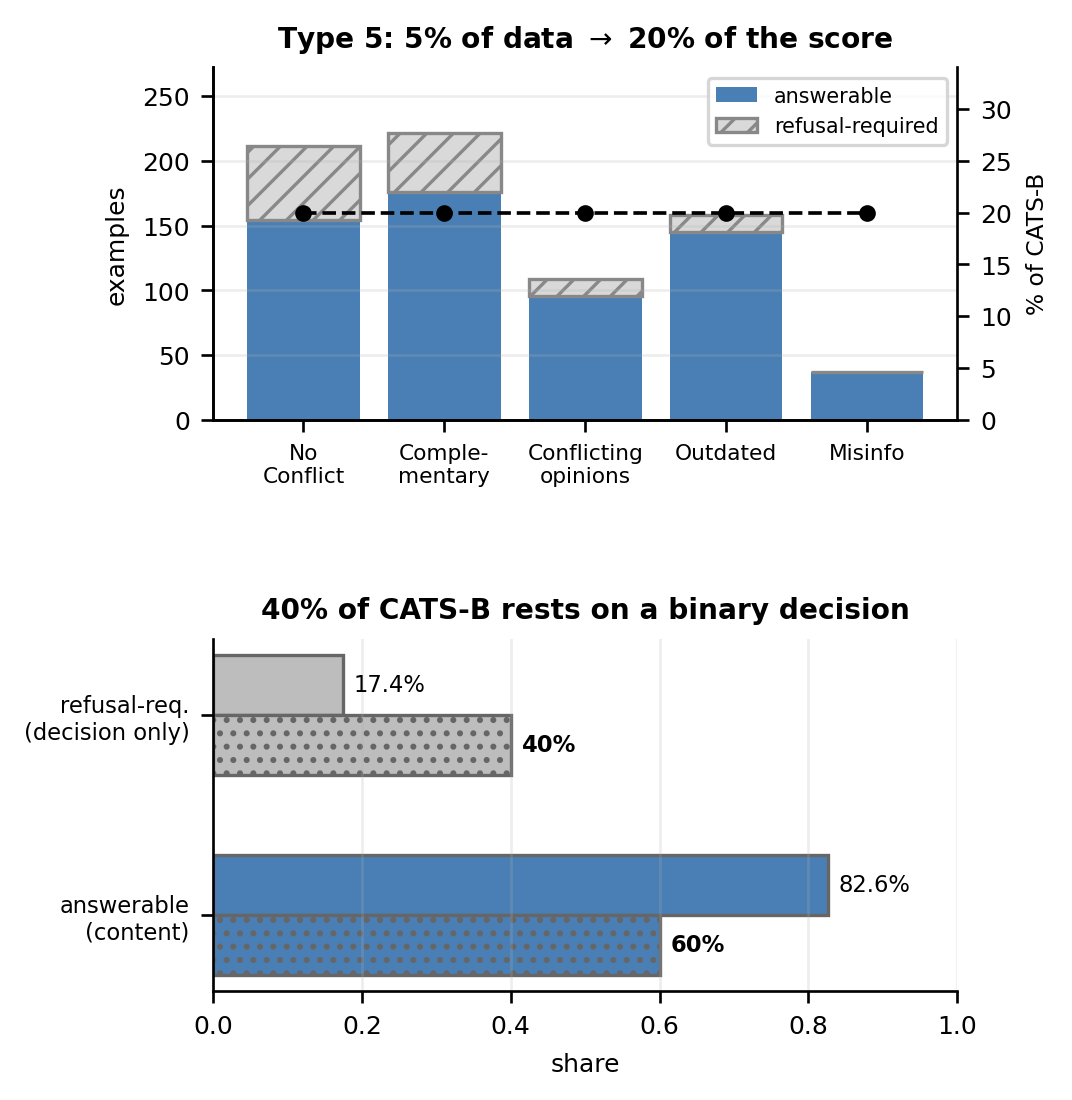
\includegraphics[height=2.842in]{figures/fig7_weight_structure.png}
\end{minipage}
\hfill
\begin{minipage}[b]{2.531in}
\centering
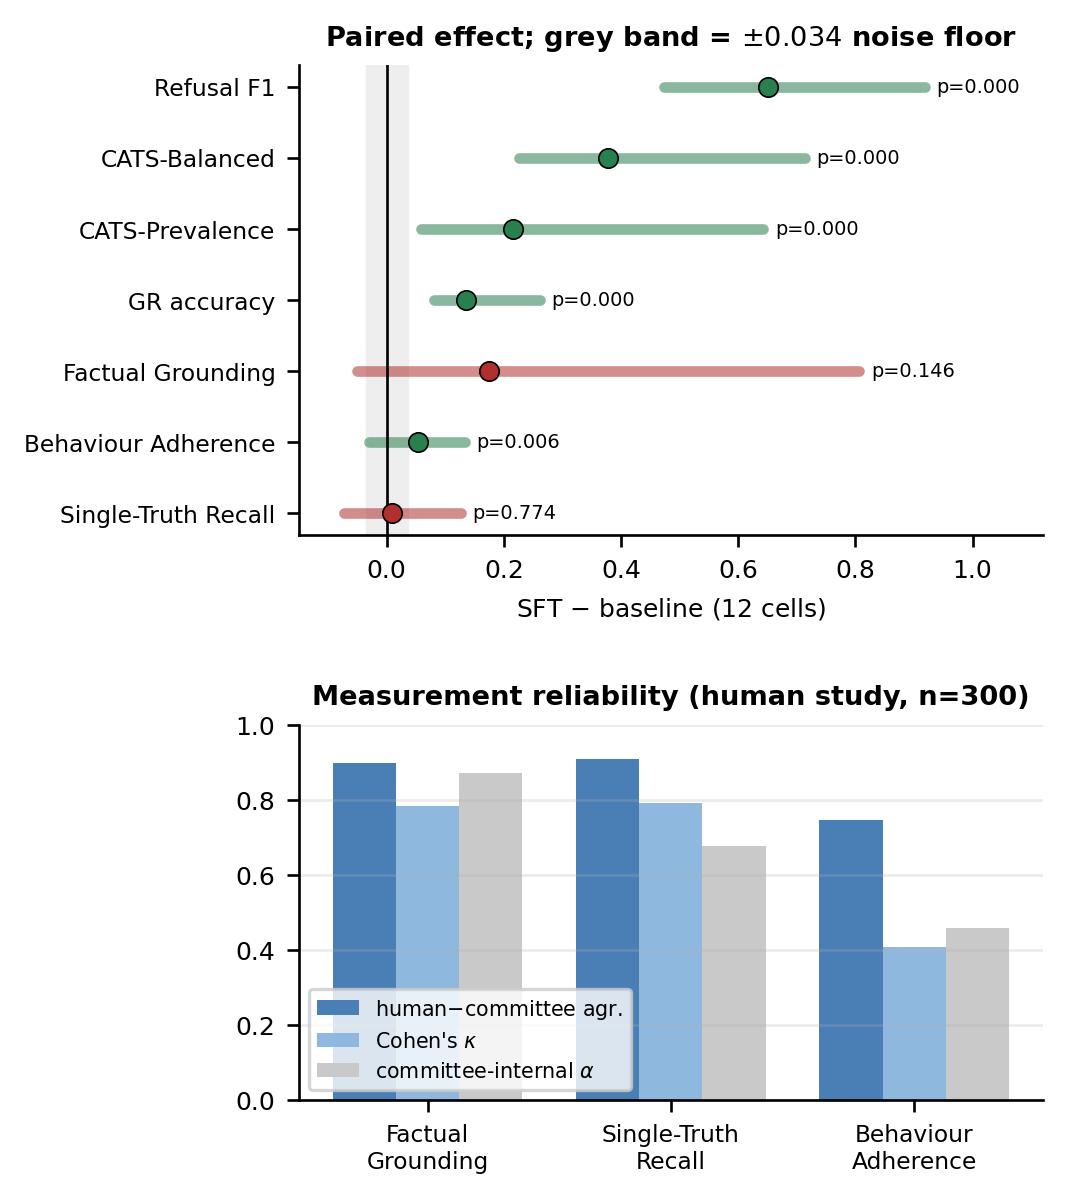
\includegraphics[height=2.842in]{figures/fig12_significance_reliability.png}
\end{minipage}
\dualcaption{figure}{fig:weights}{fig:sigrel}%
{Structural properties of the aggregate}%
{Left: paired effect of trace supervision across the twelve
end-to-end cells, with the distribution-free noise floor shaded. Right:
per-component reliability from the human study.}
\end{figure}

\section{Human Evaluation Study}
\label{app:human}

\subsection{Per-component reliability}

Four reviewers independently judged 300 generated responses, each reviewed twice,
spanning two model families, two training conditions, three prompt profiles and
all five conflict types. These 300 responses form the agreement frame on which
the human--human statistics are computed (Table~\ref{tab:human}).

\begin{table}[htbp]
\centering
\begin{minipage}[t]{0.47\linewidth}\vspace{0pt}
\centering
% Row pitch raised so this table ends level with its side-by-side partner
% (tab_judges, which has more rows); see the pair in appendix.tex.
{\tabstyle\renewcommand{\arraystretch}{2.06}\setlength{\tabcolsep}{3.5pt}
\begin{tabular*}{\linewidth}[t]{@{\extracolsep{\fill}}l rr r r@{}}\toprule
& \multicolumn{2}{c}{\textbf{human--comm.}} & \textbf{h.--h.} & \textbf{judges}\\
\cmidrule(lr){2-3}\cmidrule(lr){4-4}\cmidrule(lr){5-5}
\textbf{Component} & agr. & $\kappa$ & $\kappa$ & $\alpha$\\\midrule
FG  & 0.899 & \textbf{0.783} & 0.780 & \textbf{0.871}\\
STR & 0.908 & \textbf{0.790} & 0.773 & 0.678\\
BA  & 0.745 & 0.407 & 0.669 & 0.457\\
\bottomrule\end{tabular*}}

\end{minipage}%
\hspace{0.03\linewidth}%
\begin{minipage}[t]{0.47\linewidth}\vspace{0pt}
\centering
{\footnotesize\renewcommand{\arraystretch}{1.08}\setlength{\tabcolsep}{4.5pt}
\begin{tabular}{@{}l r rr@{}}\toprule
\textbf{Judge (behaviour)} & \textbf{prio.} & \textbf{agr.} & $\kappa$\\\midrule
anchor judge & 6 & 0.743 & 0.405\\
third judge & 2 & 0.735 & 0.339\\
second judge & 3 & 0.643 & 0.229\\
\midrule \textbf{full committee} & & \textbf{0.745} & \textbf{0.407}\\
\midrule\multicolumn{4}{@{}l}{\textit{Committee-internal agreement (300-response frame)}}\\
Factual Grounding & & $\alpha$=0.871 & 0.871\\
Single-Truth Recall & & $\alpha$=0.678 & 0.687\\
Behaviour Adherence & & $\alpha$=0.457 & 0.470\\
\bottomrule\end{tabular}}
\end{minipage}
\dualcaption{table}{tab:human}{tab:judges}%
{\textbf{Evaluator validation against independent human review.} Rows are Factual Grounding, Single-Truth Recall and Behaviour Adherence. Columns are human--committee agreement and $\kappa$, human--human $\kappa$, and \emph{judges}, the nominal $\alpha$ among the three committee models. Human--committee uses all accepted reviewer rows; human--human and \emph{judges} use the 300-response complete two-reviewer frame. The reliability ordering is identical on both instruments: grounding and recall are reliable, behaviour is not. Grounded Refusal is deterministic and therefore not judged}%
{\textbf{Per-judge agreement with human reviewers, and committee-internal agreement.} Top: each judge's behaviour agreement with human reviewers over 650 aligned judgment-level rows (the 300 two-reviewer responses plus 50 single-reviewed), alongside its configured priority. The anchor judge is empirically the best human-aligned of the three, and the full committee edges its best single member. Bottom: agreement among the three judges on the 300-response frame; the final column is mean pairwise $\kappa$.}
\end{table}

The result is a per-component reliability ordering identical on two independent
instruments, human--committee agreement and committee-internal agreement, and it
bounds what we may claim. Factual Grounding and Single-Truth Recall are reliable
($\kappa=0.78$ and $0.79$ against humans; $89.9\%$ and $90.8\%$ raw agreement).
Behaviour Adherence is not: an independent human panel agrees with the committee
on only $74.5\%$ of behaviour judgments ($\kappa=0.41$), and the three judges
agree among themselves at $\alpha=0.46$.

Consequently we treat behaviour claims differently from grounding claims. All
twelve observed BA differences lie below the human--committee disagreement rate,
so while the improvement is statistically consistent ($11/12$ cells, $p=0.006$),
we state it qualitatively and decline to interpret individual BA margins,
particularly in the misinformation regime.

The agreement frame is \textbf{300 generated responses}, each independently
reviewed by two of four reviewers, drawn from a $2\times3\times2$ design (two
model families $\times$ three prompt profiles $\times$ untuned/fine-tuned),
stratified by conflict type, with correct refusals excluded before assignment.
Reviewers judged behaviour
adherence against the per-type rubric, selected supporting documents for each
displayed claim and judged whether the response asserted the gold target;
metric pages were separated so that a factual impression could not silently
change a behaviour label.

A further 50 responses received a single review, because one reviewer completed
half an assigned queue; these carry no human--human comparison and are excluded
from the agreement frame, but their judgments are retained where a single
review suffices. No judgment is imputed. Reported statistics therefore name
their denominator explicitly, and the denominators differ by construction: the
\emph{response-level} human--human frame is 300, whereas \emph{judgment-level}
human--committee comparison pools every accepted review and so is 650
($300\times2$ complete pairs plus 50 singles). Claim-level grounding is counted
in claim units rather than responses ($477$ human--human, $1{,}029$
human--committee), and the human-consensus frame is 256 behaviour and 194
strict-recall samples.

Coverage caveats. The study covers two of the four model families and the
end-to-end condition only. Correct refusals were excluded before sampling, so the
study says nothing about refusal wording quality. The human package extracts up
to twelve claims per answer while the benchmark configuration uses eight, so
grounding denominators are aligned in logic but not identical.

\paragraph{Agreement is not uniform across the taxonomy.} Table~\ref{tab:bytype}
gives the per-conflict-type breakdown. Three patterns matter. Claim-level
grounding is near-perfect on No-conflict items ($\kappa=0.972$ human--human) and
weakest on Outdated ($\kappa=0.566$), where deciding whether a superseded
document still supports a claim is genuinely ambiguous. Human behaviour agreement
is lowest on Complementary ($\kappa=0.536$) and Outdated ($\kappa=0.505$). And
the committee's behaviour judgments track humans well on Conflicting opinions
($\kappa=0.641$) but poorly on Complementary ($\kappa=0.279$) and Misinformation
($\kappa=0.149$). Reported as a single number, behaviour reliability would hide
the fact that it is concentrated in two regimes.

\begin{table}[htbp]\centering{\small\renewcommand{\arraystretch}{1.08}\setlength{\tabcolsep}{4pt}
\begin{tabular}{@{}l cc cc cc cc@{}}\toprule
& \multicolumn{4}{c}{\textbf{human--human}} & \multicolumn{4}{c}{\textbf{human--committee}}\\
\cmidrule(lr){2-5}\cmidrule(lr){6-9}
& \multicolumn{2}{c}{Behaviour} & \multicolumn{2}{c}{FG (claims)} & \multicolumn{2}{c}{Behaviour} & \multicolumn{2}{c}{FG (claims)}\\
\cmidrule(lr){2-3}\cmidrule(lr){4-5}\cmidrule(lr){6-7}\cmidrule(lr){8-9}
\textbf{Conflict type} & agr. & $\kappa$ & agr. & $\kappa$ & agr. & $\kappa$ & agr. & $\kappa$\\\midrule
No conflict & 0.937 & 0.714 & 0.987 & 0.972 & 0.865 & \textbf{0.325} & 0.945 & 0.880\\
Complementary & 0.783 & 0.536 & 0.908 & 0.803 & 0.708 & \textbf{0.279} & 0.910 & 0.805\\
Conflicting opinions & 0.862 & 0.725 & 0.887 & 0.749 & 0.820 & 0.641 & 0.888 & 0.759\\
Outdated & 0.817 & 0.505 & 0.800 & 0.566 & 0.746 & \textbf{0.338} & 0.825 & 0.606\\
Misinformation & 0.864 & 0.725 & 0.912 & 0.821 & 0.581 & \textbf{0.149} & 0.929 & 0.855\\
\midrule \textbf{Overall} & 0.853 & 0.669 & 0.897 & 0.780 & 0.745 & 0.407 & 0.899 & 0.783\\
\bottomrule\end{tabular}}
\caption{\textbf{Agreement by conflict type.} Bold marks $\kappa<0.40$. Reliability is not uniform across the taxonomy: human reviewers agree least on Complementary and Outdated behaviour, and the committee's behaviour judgments degrade sharply on Misinformation ($\kappa=0.149$) and Complementary ($\kappa=0.279$) while remaining strong on Conflicting opinions ($\kappa=0.641$). Claim-level grounding is reliable everywhere except Outdated. Conflicting opinions is excluded from Single-Truth Recall by construction and so does not appear in that metric's strata.}
\label{tab:bytype}\end{table}

\paragraph{Per-judge and committee-internal agreement.} Table~\ref{tab:judges}
compares each judge separately against human reviewers over the 650 aligned
judgment-level rows.
The anchor judge agrees best ($0.743$ agreement, $\kappa=0.405$), the third judge
next ($0.735$, $\kappa=0.339$) and the second judge least ($0.643$,
$\kappa=0.229$); the full weighted committee reaches $\kappa=0.407$, marginally
above its best individual member. Committee-internal agreement on the
300-response frame is $\alpha=0.871$ for grounding, $0.678$ for recall and $0.457$ for
behaviour, with the behaviour spread concentrated between judge pairs (pairwise
$\kappa$ ranges from $0.368$ to $0.611$).

\paragraph{Consensus frame.} Restricting to the samples where both reviewers agree
and comparing that consensus against the committee raises agreement as expected:
behaviour $0.789$ ($\kappa=0.483$, $n=256$), strict recall $0.948$
($\kappa=0.876$, $n=194$) and claim-level grounding $0.949$ ($\kappa=0.888$,
$n=428$). Consensus filtering improves interpretability but retains easier cases
disproportionately, so we report it alongside rather than instead of the
row-level frame. The misinformation behaviour stratum does not improve under
consensus ($0.588$, $\kappa=0.165$), which confirms that its weakness is not
merely reviewer noise.

\paragraph{Alignment integrity.} Claim-level comparisons require pairing human and
committee claim inventories. All three analyses report \emph{zero} claim-alignment
issues, and all 650 accepted human reviews matched a committee judgment with no
missing matches, so no unit was dropped or approximately aligned
(Figure~\ref{fig:sigrel}).

\section{Citation Analysis}
\label{app:citation}




Few-shot Chain-of-Thought abstains at $32/128$ for Llama-3.1-8B, $38/128$ for
Qwen2.5-7B and $85/128$ for Mistral-7B, a $25$--$66\%$ spread. The exception is
worth naming rather than averaging away: Mistral-7B is also the most
abstention-prone model in the baseline end-to-end condition, so its few-shot
behaviour looks less like acquired judgment than like a prior toward refusing
that the exemplars happen to license. Chain-of-Note has the poorest citation
hygiene of any method examined, with a hard-negative citation rate roughly five
times that of the trace-tuned models. Figure~\ref{fig:comparators} contrasts the
two prompting strategies with trace supervision on answer content and on refusal
calibration.

We analyse cited-document behaviour with metrics that are not part of CATS and
do not alter any CATS component or aggregate; they are supplementary post-hoc
diagnostics computed from the same claim-level extraction used by Factual
Grounding, partitioned into a recall side (does the model cite the support
that exists?) and a precision side (is what it cites the right evidence?).

Table~\ref{tab:citdefs} defines each metric; Table~\ref{tab:citresults}
reports the changes.

\paragraph{Unit of analysis.} Every metric below is computed over
\emph{distinct cited document identifiers per claim, pooled across claims},
not raw citation mentions: if a claim cites the same document twice, that
citation is counted once for that claim. Micro-averages pool these per-claim
counts across every evaluated claim in the run rather than averaging a
per-claim rate, so claims with more citations are not down-weighted relative
to claims with fewer.

\begin{table}[htbp]
\centering
\begin{minipage}[t]{0.47\linewidth}\vspace{0pt}
\centering
{\tabstyle\setlength{\tabcolsep}{0.5pt}
\begin{tabular}[t]{@{}>{\raggedright\arraybackslash}p{0.39\linewidth} >{\raggedright\arraybackslash}p{0.33\linewidth} >{\raggedright\arraybackslash}p{0.24\linewidth}@{}}\toprule
\textbf{Metric} & \textbf{Formula} & \textbf{Unit}\\\midrule
Claim-spec.\ citation prec.\ $\uparrow$ &
$\frac{\text{approved}}{\text{all cited}}$ &
cited doc\\[5pt]
Gold-positive precision $\uparrow$ &
$\frac{\text{gold-pos.}}{\text{all cited}}$ &
cited doc\\[5pt]
Citation sufficiency $\uparrow$ &
$\frac{\text{claims w/}\geq1\text{ cite}}{\text{claims w/ support}}$ &
supported claim\\[5pt]
Soft-extra citation rate $\downarrow$ &
$\frac{\text{gold-pos., not appr.}}{\text{all cited}}$ &
cited doc\\[5pt]
Hard-negative citation rate $\downarrow$ &
$\frac{\text{not gold-pos.}}{\text{all cited}}$ &
cited doc\\[5pt]
Strict grounded, gold-clean $\uparrow$ &
$\frac{\text{gr.}\wedge\text{cit.}\wedge\text{no hard-neg.}}{\text{all claims}}$ &
extras OK\\[5pt]
Strict grounded, committee-clean $\uparrow$ &
$\frac{\text{gr.}\wedge\text{cit.}\wedge\text{clean}}{\text{all claims}}$ &
nothing OK\\
\bottomrule\end{tabular}}
\end{minipage}%
\hspace{0.03\linewidth}%
\begin{minipage}[t]{0.47\linewidth}\vspace{0pt}
\centering
% Row pitch raised so this table ends level with the definitions table beside it.
{\tabstyle\renewcommand{\arraystretch}{1.25}\setlength{\tabcolsep}{1pt}
\begin{tabular*}{\linewidth}[t]{@{\extracolsep{\fill}}>{\raggedright\arraybackslash}p{1.12in}rrr@{}}\toprule
\textbf{Metric} & \textbf{mean $\Delta$} & \textbf{min} & \textbf{max}\\\midrule
Citation sufficiency (support recall) & $+0.363$ & $-0.008$ & $+0.869$\\
Strict grounded, gold-clean & $+0.358$ & $-0.002$ & $+0.811$\\
Strict grounded, committee-clean & $+0.339$ & $+0.119$ & $+0.651$\\
Gold-positive precision & $+0.003$ & $-0.004$ & $+0.014$\\
Soft-extra citation rate & $+0.006$ & $-0.058$ & $+0.074$\\
Hard-negative citation rate & $-0.003$ & $-0.014$ & $+0.004$\\
Claim-specific citation precision & $-0.003$ & $-0.077$ & $+0.055$\\
\bottomrule\end{tabular*}}
\end{minipage}
\dualcaption{table}{tab:citdefs}{tab:citresults}%
{\textbf{Citation-metric definitions.} ``Approved'' means the cited
document is in the committee's claim-specific support set; ``gold-positive''
means its gold per-document verdict is \textit{supports} or \textit{partially
supports}, independent of which specific claim is being checked; ``clean''
means no soft-extra and no hard-negative citation. The two strict-grounded
rates share a base condition (committee-grounded, cited) and differ only in
what they tolerate: the gold-clean rate forbids hard negatives but allows
soft extras, the committee-clean rate forbids both, making it the single most
demanding number in this section. $\uparrow$/$\downarrow$ after the metric
name marks whether higher or lower is the better direction. All fractions
count distinct cited documents or evaluated claims as noted in the Unit
column}%
{Citation-metric changes under trace supervision, fine-tuned minus
baseline, across the twelve end-to-end cells.}
\end{table}

Only the recall side moves. The strict committee-clean metric, which requires a
claim to be committee-supported, cited and free of both extraneous and
incorrect citations, is positive in all twelve cells and is the single most
demanding citation number we report.

\FloatBarrier

Two further observations. Untuned models under minimal prompts post
\emph{higher} claim-specific citation precision than their own fine-tuned
counterparts in all four cases ($0.736$--$0.867$ against $0.713$--$0.800$)
while citing almost nothing (recall $0.036$--$0.139$): precision over a
near-empty denominator, not a quality signal.
And the recall-side metrics correlate with Factual Grounding at
$\rho=0.93$--$0.98$, so they are largely redundant with it, whereas every
precision-side metric sits at $|\rho|\leq0.46$ against every CATS component and
therefore carries information the framework does not otherwise capture. Behaviour
Adherence is the CATS component least related to citation behaviour, which is an
independent check that its orthogonality requirement holds in practice.
Figure~\ref{fig:cit1} plots the sufficiency and precision trajectories across
the instruction ladder, and Figure~\ref{fig:cit2} shows the precision paradox
directly.





\FloatBarrier

\begin{figure}[htbp]
\centering
\begin{minipage}[b]{1.840in}
\centering
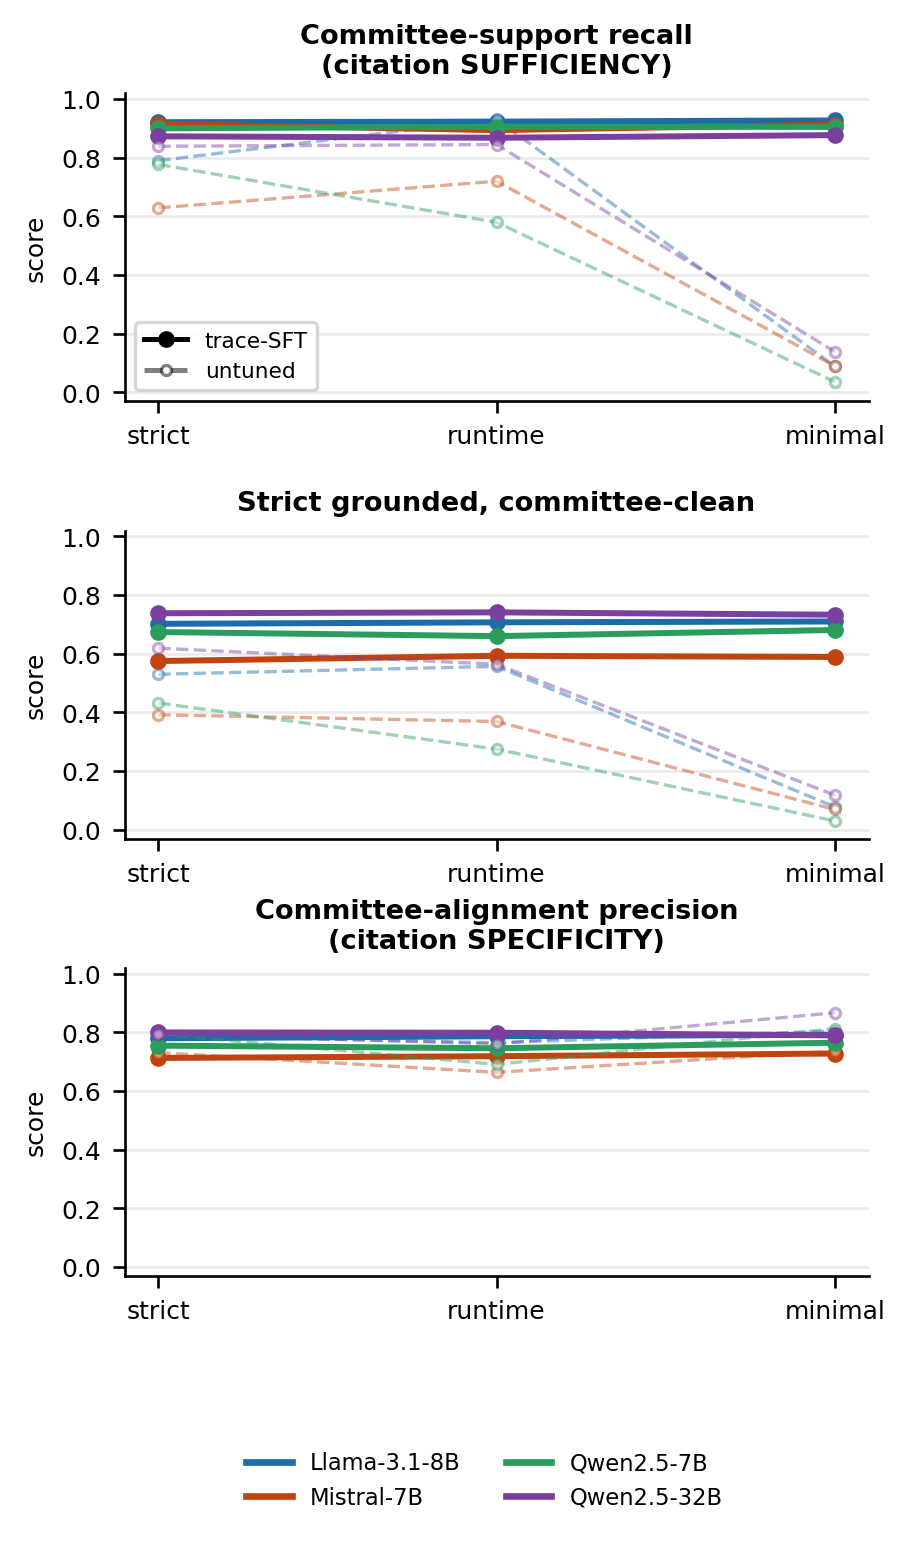
\includegraphics[height=3.121in]{figures/fig8_citation_sufficiency.png}
\end{minipage}
\hfill
\begin{minipage}[b]{3.460in}
\centering
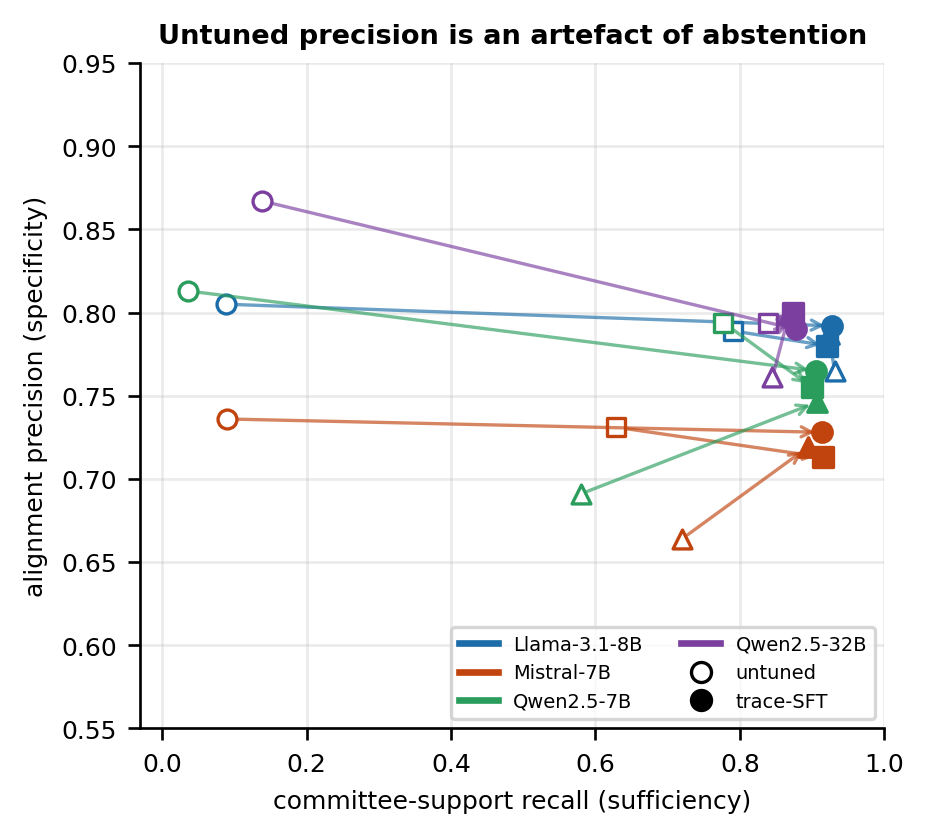
\includegraphics[height=3.121in]{figures/fig9_precision_paradox.png}
\end{minipage}
\dualcaption{figure}{fig:cit1}{fig:cit2}%
{Trace supervision fixes citation sufficiency, not citation
precision}%
{The precision paradox: untuned precision is an artefact of
abstention from citing. Every model moves down-and-right when fine-tuned.}
\end{figure}

\begin{figure}[htbp]
    \centering
    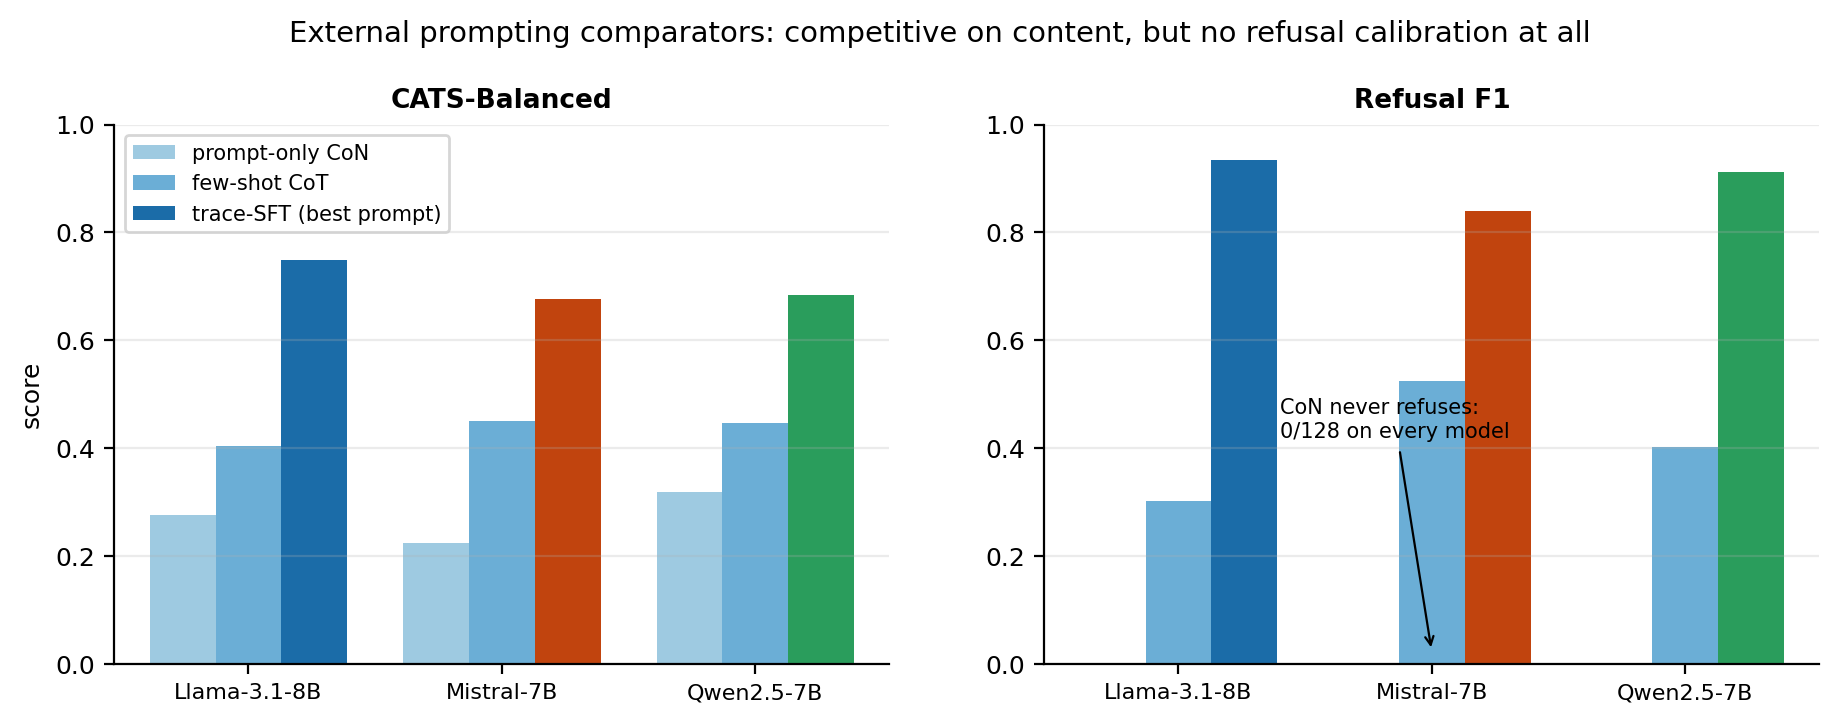
\includegraphics[width=0.95\textwidth]{figures/fig6_comparators.png}
    \caption{External prompting comparators. Both prompting-only strategies reach
    competitive answer content but neither acquires refusal calibration:
    Chain-of-Note records $0/128$ correct refusals on every model.}
    \label{fig:comparators}
\end{figure}

\section{Bounding Factual Grounding}
\label{app:deconfound}

The \emph{lower} bound includes the missed refusals; the \emph{upper} bound
restricts to the like-for-like population where the model answered \emph{and} the
gold label is answerable. The intervals separate in all four minimal-prompt cells
and in only two others (Qwen2.5-7B runtime, Mistral-7B strict). Instruction
volume is also not monotonically helpful for baseline models: grounding is higher
under the shorter runtime prompt than the strict one in all four families, and in
the extreme case Llama-3.1-8B reaches $\mathrm{FG}=0.897$ while correctly
refusing $2$ of $128$ refusal-required items, so its grounding is computed over a
markedly easier population.

Reported Factual Grounding is averaged over
$\textit{fg\_n}=608+\textit{missed refusals}$, so run types that refuse at
different rates are not scored on the same population. Table~\ref{tab:fgdenom}
gives both bounds per cell: the reported value, which includes missed refusals,
and the like-for-like interval restricted to examples the model answered and the
gold label marks answerable. Figure~\ref{fig:fgdenom} plots both, alongside the
model-dependence of the denominator itself.



\begin{table}[htbp]
\centering
\begin{minipage}[t]{0.84\linewidth}\vspace{0pt}
\centering
{\scriptsize\renewcommand{\arraystretch}{1.0}\setlength{\tabcolsep}{1.6pt}
\begin{tabular}{@{}ll cc cc c@{}}\toprule
& & \multicolumn{2}{c}{\textbf{reported FG}} & \multicolumn{2}{c}{\textbf{like-for-like FG}} & \\
\cmidrule(lr){3-4}\cmidrule(lr){5-6}
\textbf{Model} & \textbf{Prompt} & base & \textsc{sft} & base & \textsc{sft} & \textbf{sep.}\\\midrule
Qwen2.5-7B & strict & 0.617 & 0.838 & [0.81,0.92] & [0.86,0.87] & --\\
 & runtime & 0.651 & 0.829 & [0.69,0.85] & [0.85,0.86] & \ding{51}\\
 & minimal & 0.031 & 0.837 & [0.00,0.04] & [0.86,0.88] & \ding{51}\\
\addlinespace[2pt]
Qwen2.5-32B & strict & 0.851 & 0.812 & [0.84,1.00] & [0.85,0.85] & --\\
 & runtime & 0.864 & 0.814 & [0.86,1.00] & [0.85,0.85] & --\\
 & minimal & 0.108 & 0.822 & [0.00,0.13] & [0.86,0.86] & \ding{51}\\
\addlinespace[2pt]
Llama-3.1-8B & strict & 0.705 & 0.852 & [0.75,0.94] & [0.88,0.88] & --\\
 & runtime & 0.897 & 0.849 & [0.88,1.00] & [0.87,0.88] & --\\
 & minimal & 0.074 & 0.857 & [0.00,0.09] & [0.88,0.88] & \ding{51}\\
\addlinespace[2pt]
Mistral-7B & strict & 0.624 & 0.796 & [0.58,0.74] & [0.87,0.87] & \ding{51}\\
 & runtime & 0.739 & 0.762 & [0.71,0.90] & [0.83,0.83] & --\\
 & minimal & 0.079 & 0.792 & [0.00,0.10] & [0.86,0.86] & \ding{51}\\
\addlinespace[2pt]
\bottomrule\end{tabular}}
\end{minipage}

\vspace{8pt}

\begin{minipage}[t]{0.56\linewidth}\vspace{0pt}
\centering
{\scriptsize\renewcommand{\arraystretch}{2.52}\setlength{\tabcolsep}{3pt}
\begin{tabular}{@{}l@{\hspace{4pt}} cc cc@{}}\toprule
& \multicolumn{2}{c}{\textbf{Min.\ FG}} & \multicolumn{2}{c}{\textbf{Spread}}\\
\cmidrule(lr){2-3}\cmidrule(lr){4-5}
\textbf{Model} & base & \textsc{sft} & base & \textsc{sft}\\\midrule
Qwen-7B & 0.031 & \textbf{0.837} & 0.442 & \textbf{0.026}\\
Qwen-32B & 0.108 & \textbf{0.822} & 0.398 & \textbf{0.009}\\
Llama-8B & 0.074 & \textbf{0.857} & 0.345 & \textbf{0.016}\\
Mistral-7B & 0.079 & \textbf{0.792} & 0.278 & \textbf{0.020}\\
\bottomrule\end{tabular}}
\end{minipage}
\dualcaption{table}{tab:fgdenom}{tab:internalization}%
{\textbf{The Factual-Grounding denominator is model-dependent.} $\textit{fg\_n}=608+\textit{missed refusals}$, so a baseline model that rarely refuses is additionally scored on ${\sim}130$ refusal-required items whose evidence is insufficient by construction, while its false abstentions enter the denominator at $\mathrm{FG}=0$. The \emph{like-for-like} columns bound FG on the population where the model answered \emph{and} the gold label is answerable. A check mark marks cells where the fine-tuned interval lies strictly above the baseline interval: this holds in every minimal-prompt cell and in none of the strict cells}%
{\textbf{Internalization.} Factual Grounding under the minimal prompt, and the spread of CATS-Balanced across the strict/runtime/minimal ladder. Baseline grounding collapses without scaffolding and baseline behaviour swings an order of magnitude more across the ladder.}
\end{table}

\begin{figure}[htbp]
    \centering
    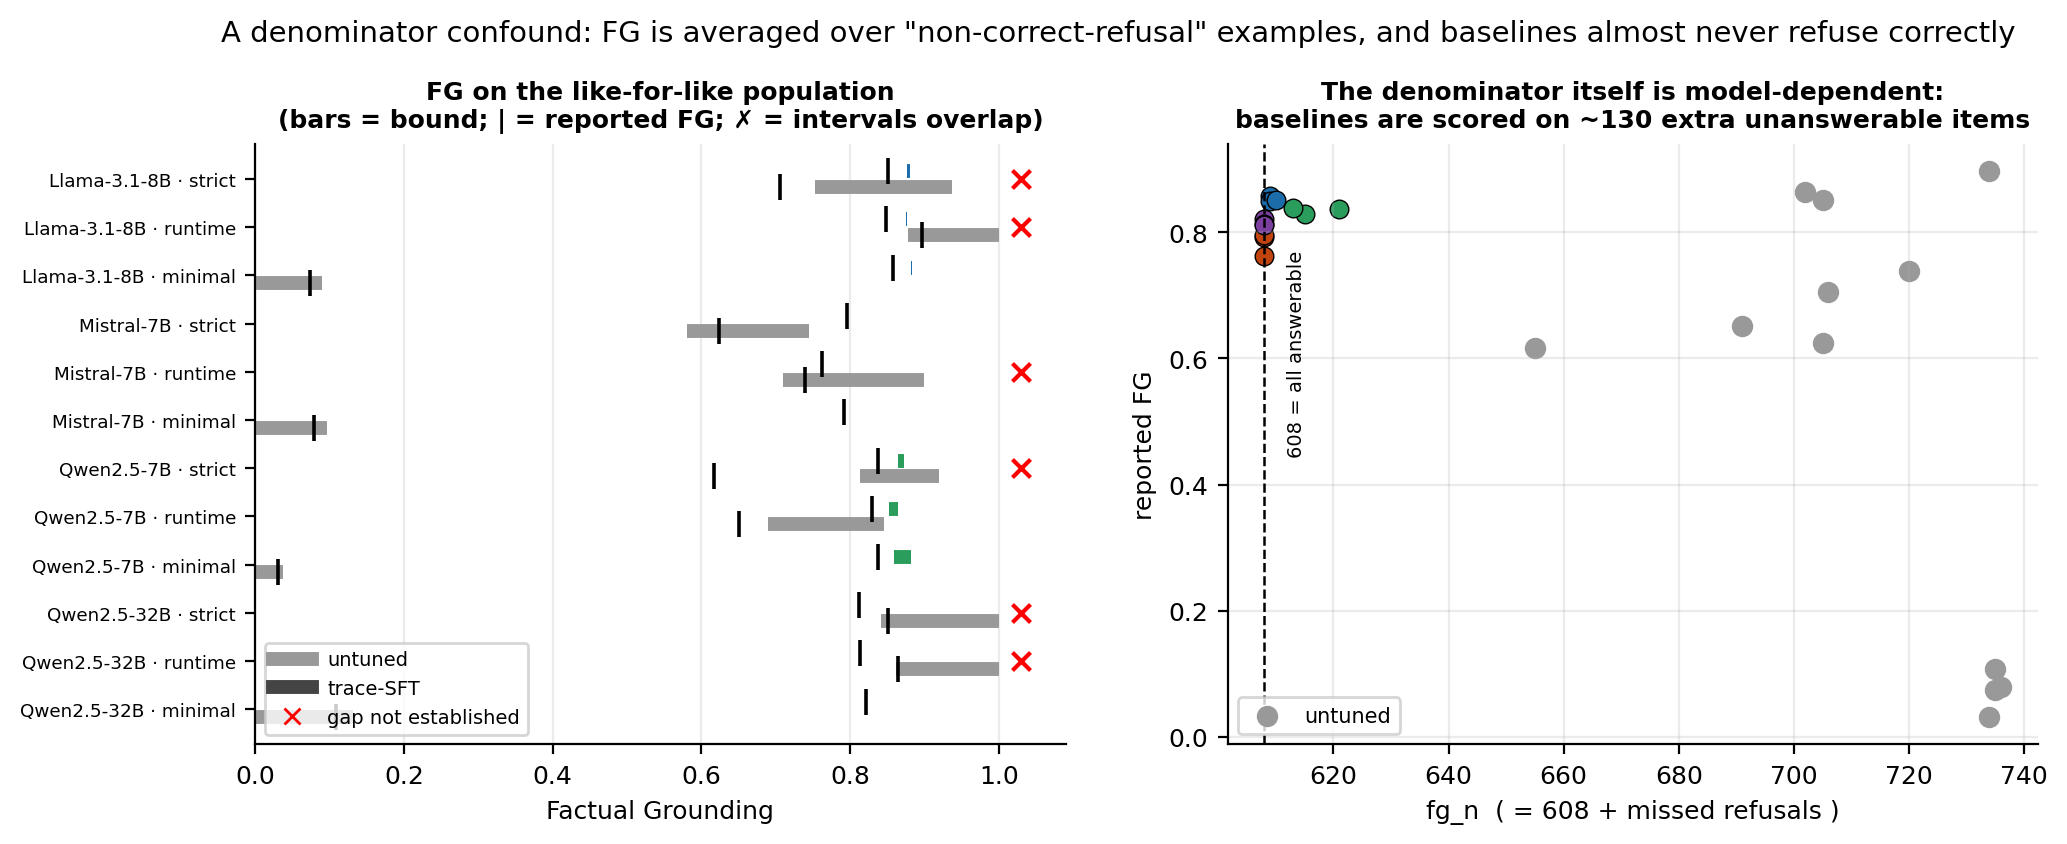
\includegraphics[width=0.95\textwidth]{figures/fig11_fg_denominator.png}
    \caption{The Factual-Grounding denominator confound. Left: FG on the
    like-for-like population, with bars giving the bound and vertical marks the
    reported value; crosses mark cells where the intervals overlap and no gap is
    established. Right: the denominator $\textit{fg\_n}=608+\textit{missed
    refusals}$ is itself model-dependent, so baseline models are scored on up to
    ${\sim}130$ extra items whose evidence is insufficient by construction.}
    \label{fig:fgdenom}
\end{figure}

\section{Additional Figures and Tables}
\label{app:figs}

\begin{figure}[htbp]
\centering
\begin{minipage}[b]{1.756in}
\centering
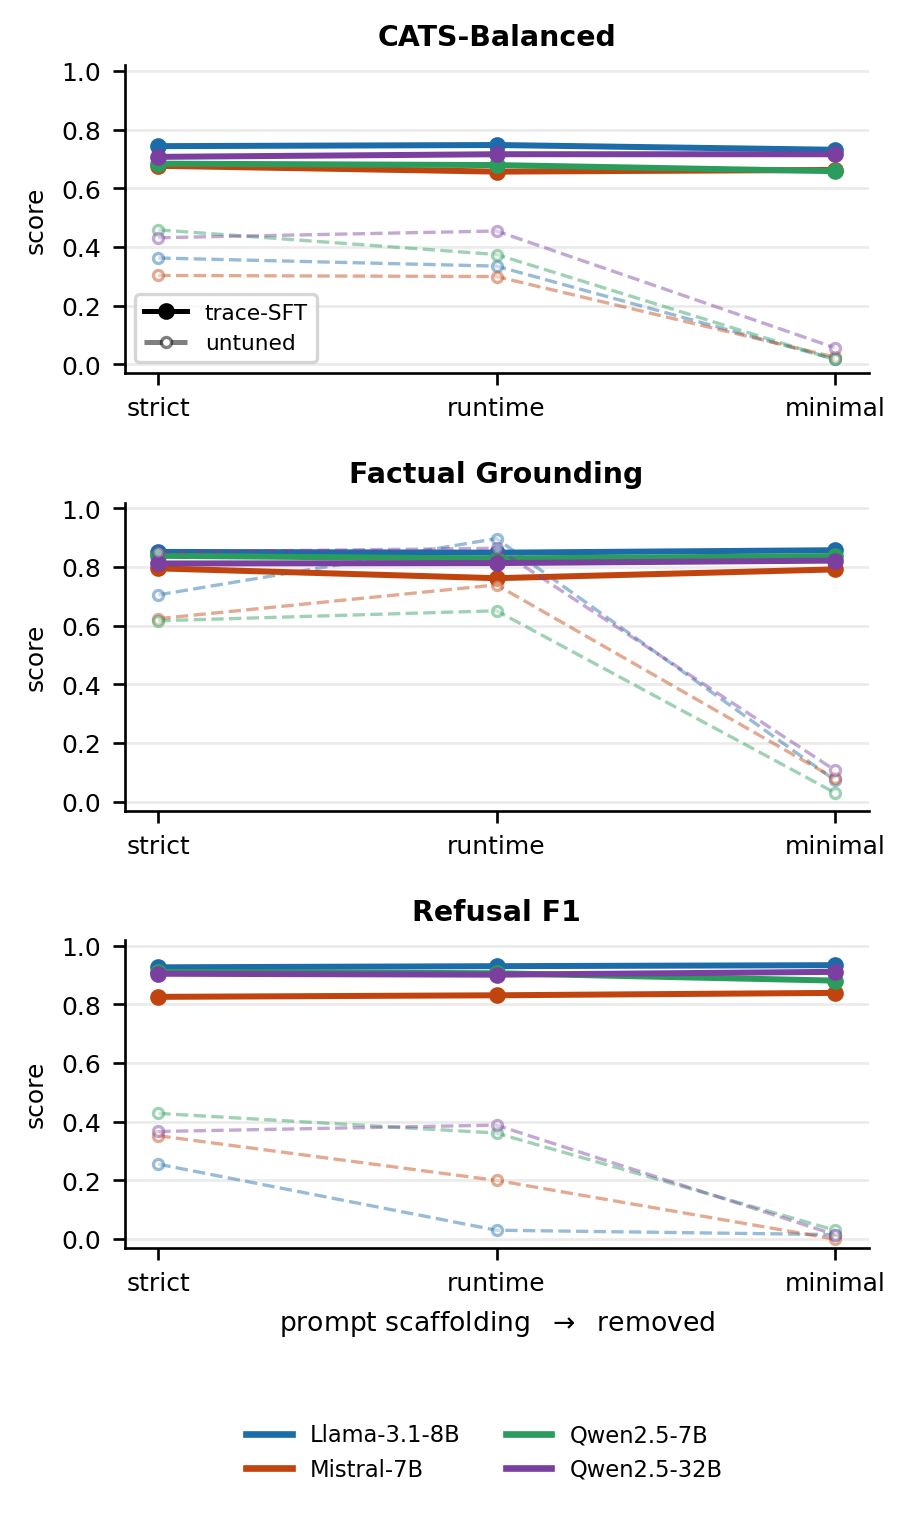
\includegraphics[height=2.925in]{figures/fig1_internalization.png}
\end{minipage}
\hfill
\begin{minipage}[b]{3.544in}
\centering
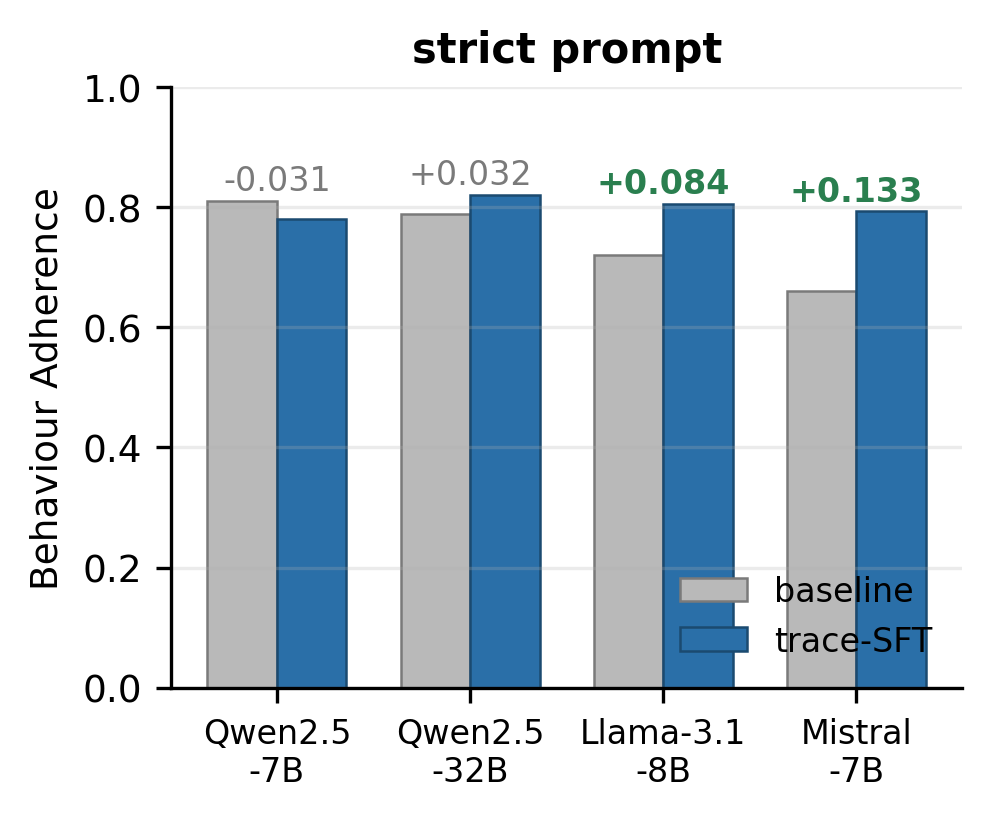
\includegraphics[height=2.925in]{figures/fig16_ba_strict.png}
\end{minipage}
\dualcaption{figure}{fig:internal}{fig:bastrict}%
{Behaviour across the prompt ladder. Solid lines are trace-tuned
models, dashed lines untuned. Fine-tuned behaviour is essentially flat as the
instruction is stripped away; untuned grounding and refusal collapse}%
{Behaviour Adherence under the \textbf{strict} prompt, baseline
against trace-tuned. Deltas are annotated; bold green marks a gain exceeding
the $\pm0.034$ noise floor.}
\end{figure}

\subsection{Behaviour Adherence by prompt condition}

Figures~\ref{fig:bastrict} and~\ref{fig:baminimal} give the per-model Behaviour
Adherence scores behind the summary in \S\ref{sec:refusal}, separated by
instruction strength. Two patterns are visible that the aggregate range hides.
Under the strict prompt the gain is strongly ordered by how well the baseline
already follows instructions: Mistral-7B starts lowest ($0.660$) and gains most
($+0.133$), Llama-3.1-8B gains $+0.084$, while the two Qwen baselines already sit
at $0.789$ and $0.811$ and move $+0.032$ and $-0.031$. Only the first two clear
the $\pm0.034$ noise floor, so on the strict prompt trace supervision is best read
as closing a gap for weaker instruction-followers rather than as lifting every
model.

Under the minimal prompt the picture is more uniform. Every model gains
($+0.031$ to $+0.062$) and the baselines compress into a narrow band
($0.727$--$0.747$), because a forty-word instruction that never names the
taxonomy removes the advantage the stronger instruction-followers had. The
Qwen2.5-7B cell that regresses under strict prompting turns positive here. This
is the same internalization effect \S\ref{sec:internalization} reports, seen on a
single component: what the strict prompt supplies externally, trace supervision
supplies internally, so the two conditions converge for tuned models and diverge
for baselines. Because Behaviour Adherence is the least reliable CATS component
($\kappa=0.41$ against human review, \S\ref{sec:human}), these per-cell margins
should be read as directional rather than as point estimates.

\begin{figure}[htbp]
\centering
\begin{minipage}[b]{2.766in}
\centering
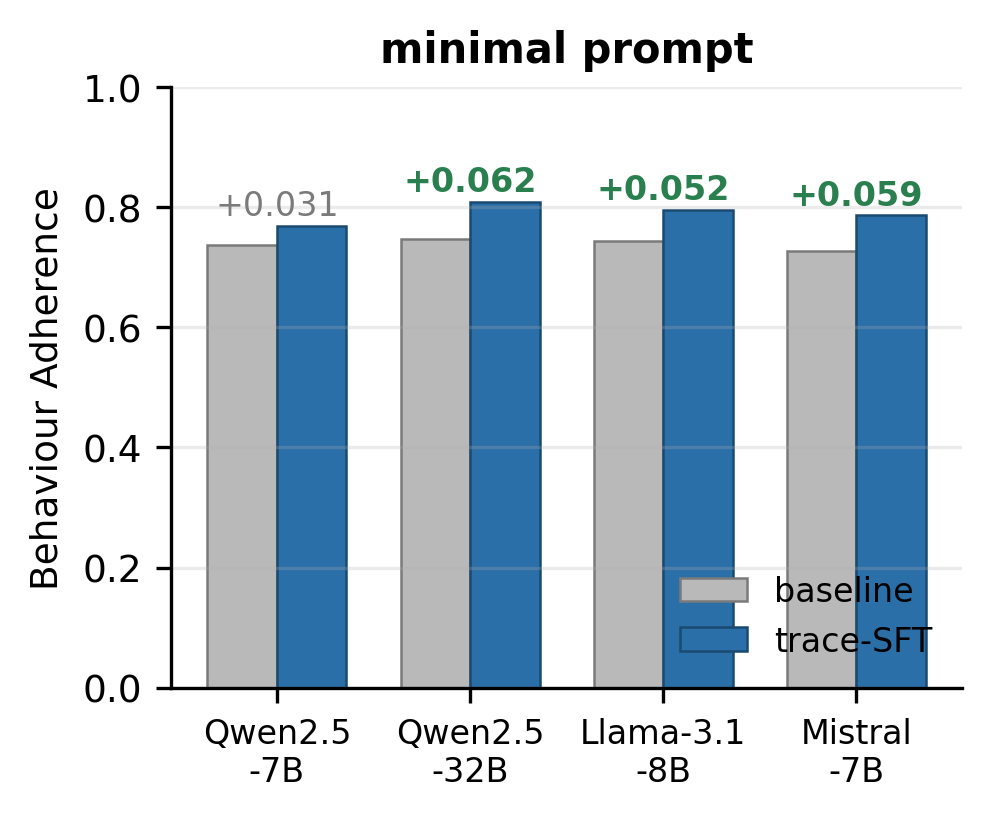
\includegraphics[height=2.283in]{figures/fig17_ba_minimal.png}
\end{minipage}
\hfill
\begin{minipage}[b]{2.534in}
\centering
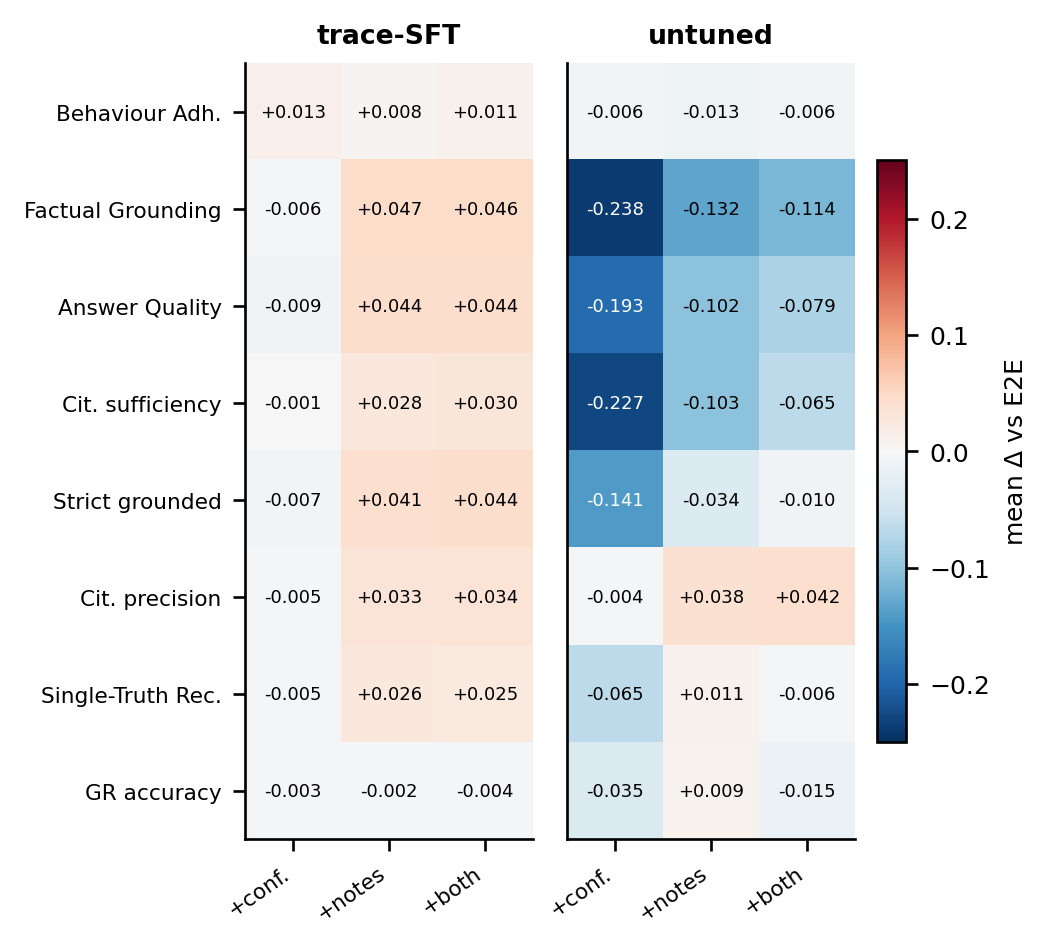
\includegraphics[height=2.283in]{figures/fig13_oracle_heatmap.png}
\end{minipage}
\dualcaption{figure}{fig:baminimal}{fig:oracleheat}%
{Behaviour Adherence under the \textbf{minimal} prompt. Baselines
compress into a narrow band once the instruction no longer names the
taxonomy, and every model gains}%
{Mean effect of each oracle on every metric. Fine-tuned models gain
on the targeted metrics; untuned models are harmed uniformly, most severely
on grounding under the conflict-label oracle.}
\end{figure}


The flatness is a property of the whole ladder, not only its endpoints: across
all twenty model$\times$metric cells the intermediate runtime condition never
falls more than $0.030$ outside the strict--minimal interval for a trace-tuned
model, inside the $\pm0.034$ noise floor. Single-truth recall shows the same
pattern, with baseline spreads of $0.047$--$0.196$. The result also reproduces on
measurements never part of CATS: analysing cited-document behaviour separately
(Appendix~\ref{app:citation}), baseline citation sufficiency swings by $0.730$
across the prompt ladder while fine-tuned sufficiency swings by $0.011$, a factor
of roughly seventy, on an instrument built after and independently of the
framework whose claim it corroborates.





\section{Oracle Ablations: Full Results}
\label{app:oracle}



\begin{table}[htbp]\centering{\small\renewcommand{\arraystretch}{1.06}\setlength{\tabcolsep}{5.5pt}
\begin{tabular}{@{}l@{\extracolsep{\fill}} ccc ccc ccc@{}}\toprule
& \multicolumn{3}{c}{\textbf{+ gold conflict label}} & \multicolumn{3}{c}{\textbf{+ gold per-doc notes}} & \multicolumn{3}{c}{\textbf{+ both}}\\
\cmidrule(lr){2-4}\cmidrule(lr){5-7}\cmidrule(lr){8-10}
\textbf{Metric} & mean $\Delta$ & $+/n$ & $p$ & mean $\Delta$ & $+/n$ & $p$ & mean $\Delta$ & $+/n$ & $p$\\\midrule
Behaviour Adherence & \textbf{+0.013} & 8/9 & \textbf{0.039} & +0.008 & 10/12 & \textbf{0.039} & +0.011 & 9/12 & 0.146\\
Factual Grounding & -0.006 & 3/9 & 0.508 & \textbf{+0.047} & 12/12 & \textbf{0.000} & \textbf{+0.046} & 12/12 & \textbf{0.000}\\
Answer Quality & -0.009 & 2/9 & 0.180 & \textbf{+0.044} & 12/12 & \textbf{0.000} & \textbf{+0.044} & 12/12 & \textbf{0.000}\\
Citation sufficiency & -0.001 & 3/9 & 0.508 & \textbf{+0.028} & 12/12 & \textbf{0.000} & \textbf{+0.030} & 12/12 & \textbf{0.000}\\
Strict grounded (cit.) & -0.007 & 3/9 & 0.508 & \textbf{+0.041} & 12/12 & \textbf{0.000} & \textbf{+0.044} & 12/12 & \textbf{0.000}\\
Citation precision & -0.005 & 2/9 & 0.180 & \textbf{+0.033} & 12/12 & \textbf{0.000} & \textbf{+0.034} & 12/12 & \textbf{0.000}\\
Single-Truth Recall & -0.005 & 3/9 & 0.508 & +0.026 & 9/12 & 0.146 & +0.025 & 8/12 & 0.388\\
Decision accuracy & -0.003 & 2/9 & 0.180 & -0.002 & 5/12 & 0.774 & -0.004 & 5/12 & 0.774\\
\bottomrule\end{tabular}}
\caption{\textbf{Mechanism-matched oracle ablations (fine-tuned models).} Each intervention supplies gold information for one reasoning stage; a metric is \emph{targeted} if it depends on that stage. The gold conflict label moves Behaviour Adherence and nothing else; the gold per-document notes move every grounding and citation metric in $9/9$ cells and leave the answer/refusal decision untouched. $p$ is an exact two-sided sign test over model$\times$prompt cells. Qwen2.5-32B is excluded from the conflict-oracle columns because of the scoring artifact documented in Appendix~\ref{app:artifacts}; the $+/n$ column reports the exact number of cells contributing to each test ($n=9$ for the conflict oracle, $n=12$ otherwise).}
\label{tab:oracle}\end{table}

\subsection{Additivity, exceptions and baseline behaviour}

Over the cells common to all three oracle conditions, the residual
$|\Delta_{\text{both}}-(\Delta_{\text{conflict}}+\Delta_{\text{notes}})|$ is at
most $0.012$ on every grounding metric. Behaviour is the single exception, with a
residual of $-0.014$: supplying both oracles yields \emph{less} behavioural gain
than the conflict label alone, consistent with the long injected notes block
competing for attention with the label the model is asked to reproduce.

Two caveats keep the claim honest. The effects are small in absolute terms, so it
is their \emph{consistency} across cells rather than their magnitude that carries
the evidence. And supplying perfect Stage-1 \emph{and} Stage-2 information still
leaves most of the residual error in place, which locates that error in Stage-3
synthesis, in gold-annotation noise, or in judge strictness; we have not
separated those three.

For baseline models every oracle \emph{hurts}, and the conflict label is
catastrophic for grounding ($-0.238$; Figure~\ref{fig:oracleheat}). The same
injected information is informative for a trace-tuned model and harmful for a
baseline one, which is a caution against reading oracle numbers as upper bounds
on what prompting alone can achieve.

\begin{figure}[htbp]
    \centering
    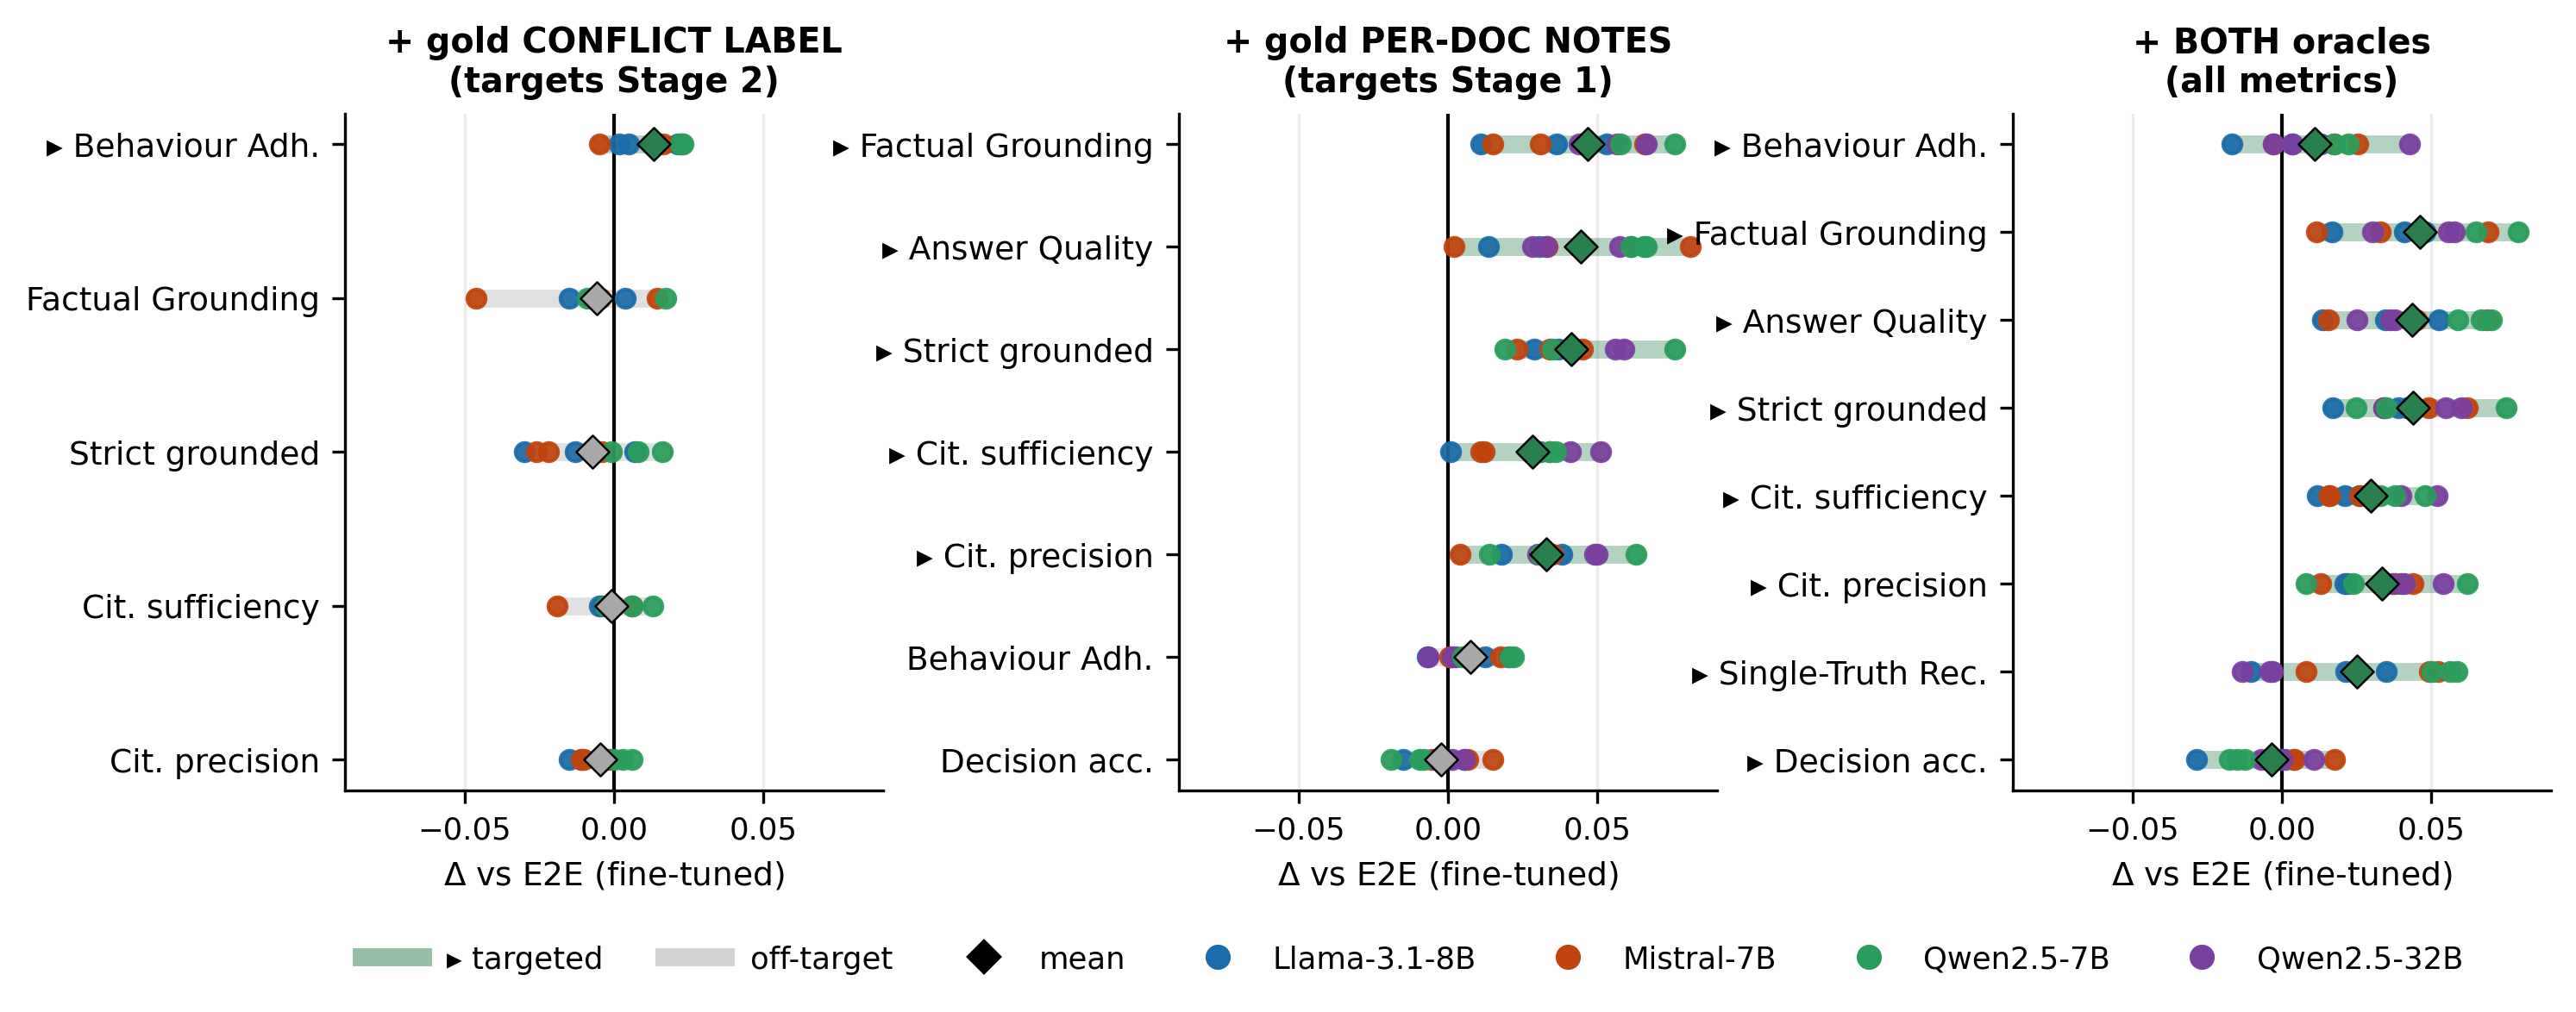
\includegraphics[width=0.95\textwidth]{figures/fig5_oracle_mechanism.png}
    \caption{Each oracle moves the metric it targets and essentially nothing
    else. Green bars are targeted metrics, grey bars are specificity controls;
    diamonds mark means, points individual model$\times$prompt cells.}
    \label{fig:oraclefig}
\end{figure}

\section{Excluded Rows and Diagnostics}
\label{app:artifacts}

Three rows are excluded from all reporting: Qwen2.5-32B, conflict-oracle,
all three prompts. Factual Grounding collapses to $0.0016$--$0.0047$ while
Behaviour Adherence ($\approx0.82$) and Single-Truth Recall ($\approx0.75$) stay
normal, against FG of $0.81$--$0.88$ for the same model elsewhere, a roughly
two-hundred-fold drop isolated to one cell. Normal behaviour and recall with near-zero grounding means the model produced
adequate, fact-containing answers whose claim-level citation linkage went
unrecovered by the scorer; the independently computed citation metrics for these
runs are ordinary, localising the fault to grounding extraction rather than
generation. Because answer quality fuses geometrically with FG, these rows
also yield the aggregate floor of exactly $0.400$
(Appendix~\ref{app:aggregate}). We exclude Qwen2.5-32B from both run types
here so baseline and fine-tuned comparisons remain balanced.

Separately, three benchmark records carry a numeric conflict identifier
disagreeing with their authoritative textual label; applicability from the
numeric field would give a single-truth denominator of 484 rather than 487.
Every reported run shows 487, so no result is affected.

\section{Released Artifacts}
\label{app:annprompts}

We release the full resource and the prompt suite used to build and evaluate it.
The release comprises: the \textbf{training/validation split} (943 examples) and
the \textbf{held-out benchmark} (736 examples), together carrying $10{,}343$
adjudicated evidence units, each with a per-document verdict, an extracted key
fact, a snippet-anchored supporting quote, a verdict rationale, a source-quality
label and the complete annotator vote tally; the \textbf{stagewise annotation
prompts} (system prompt and user template for each of the three annotation
stages), which define the annotation contract described in
Appendix~\ref{app:annotation}; the \textbf{end-to-end inference prompts} for all
three instruction strengths; the \textbf{CATS judge prompts}; and the per-run
evaluation outputs from which every number in this paper is computed.

Records are distributed as JSONL with dataset cards documenting per-source
provenance and the upstream licence for each source family. All artifacts are
available at \url{https://anonymous.4open.science/r/rag_reason-2F8F/}.

\section{End-to-End Inference Prompts}
\label{app:e2eprompts}

\subsection{Why the prompt is varied}

Varying the prompt is what makes it testable whether conflict-aware behaviour has
been \emph{learned} or is merely being \emph{recited} from the instruction. A
model that produces the trace only when the strict prompt describes it may be
following the prompt; a model that still produces it under the minimal prompt,
which never mentions the trace, the taxonomy or the citation format, has learned
a mapping from retrieval context to behaviour. Training and evaluating across all
three variants is therefore an instrument, not a data-augmentation trick, and
\S\ref{sec:internalization} reports the resulting gap.

The three end-to-end instruction strengths are reproduced verbatim below. Each
condition is a system prompt plus a user template; the placeholders are filled
with the query and the retrieved documents at generation time. Only typographic
normalisation was applied for inclusion here and no wording was changed.

The ladder is a controlled reduction in \emph{instruction}, not in task. The
underlying evidence problem, the retrieved set and the expected target are
identical across the three; what changes is how much of the procedure the prompt
restates (Table~\ref{tab:promptladder}):

\begin{table}[htbp]\centering{\tabstyle\setlength{\tabcolsep}{3pt}
\begin{tabular*}{\linewidth}{@{\extracolsep{\fill}}l@{}}\toprule
\textbf{Condition, length and what the prompt still states}\\\midrule
\textbf{strict} --- $1{,}965$ words ($49\times$)\\
\hspace{1em}full taxonomy, verdict heuristics, threshold and\\
\hspace{1em}edge-case rules, citation policy, output contract\\[3pt]
\textbf{runtime} --- $195$ words ($5\times$)\\
\hspace{1em}three-stage schema, allowed labels, abstention\\
\hspace{1em}and composition rules, citations, sentinel\\[3pt]
\textbf{minimal} --- $40$ words ($1\times$)\\
\hspace{1em}evidence-only answering and when to abstain.\\
\hspace{1em}Nothing else\\
\bottomrule\end{tabular*}}
\caption{The three end-to-end instruction strengths, measured by system-prompt
length.}
\label{tab:promptladder}
\end{table}

The minimal system prompt is four sentences long and \emph{never mentions} the
evidence trace, the three stages, the conflict taxonomy, the citation format or
the terminating sentinel. A fine-tuned model nonetheless emits all of them, which
is what \S\ref{sec:internalization} measures: behaviour under this prompt is the
internalization probe, and the collapse of untuned grounding here
($0.031$--$0.108$) against fine-tuned grounding ($0.792$--$0.857$) is a comparison
between models given \emph{these forty words} and nothing more.

Two details in the strict prompt are worth flagging because they are referenced
elsewhere. It requires citations on at least $80\%$ of answer sentences, whereas
the evaluator marks a citation pass at $75\%$; the specification and the scoring
threshold are related but not identical, and we report both rather than eliding
the gap. It also asks the model to order cited documents by the source-quality
label it assigned in Stage~1, which is one route by which the URL-whitelist
heuristic of Appendix~\ref{app:annotation} can influence answer composition.

The three oracle conditions of \S\ref{sec:oracle} use the same three instruction
strengths with an additional block injecting the gold conflict label, the gold
per-document notes, or both. Those twelve further templates are released with the
artifacts but are not reproduced here, since they differ from the corresponding
end-to-end prompt only by the injected block and the instruction to preserve it.

\subsection{Strict}
\PromptFile{Strict system prompt (\texttt{system\_e2e.txt})}{inference_prompts/system_e2e.txt}
\PromptFile{Strict user template (\texttt{user\_e2e.txt})}{inference_prompts/user_e2e.txt}

\subsection{Runtime}
\PromptFile{Runtime system prompt (\texttt{system\_e2e\_runtime.txt})}{inference_prompts/system_e2e_runtime.txt}
\PromptFile{Runtime user template (\texttt{user\_e2e\_runtime.txt})}{inference_prompts/user_e2e_runtime.txt}

\subsection{Minimal}
\PromptFile{Minimal system prompt (\texttt{system\_e2e\_minimal.txt})}{inference_prompts/system_e2e_minimal.txt}
\PromptFile{Minimal user template (\texttt{user\_e2e\_minimal.txt})}{inference_prompts/user_e2e_minimal.txt}

\FloatBarrier

\section{CATS Judge Prompts}
\label{app:catsprompts}

The complete active judge bundle is reproduced verbatim below: one shared system
message, the three task prompts, and the five-type behaviour rubric that the
Behaviour Adherence prompt selects from. Placeholders in braces are filled at
evaluation time. Only typographic normalisation was applied.

This is the \emph{entire} bundle. Grounded Refusal has no prompt because it is
computed deterministically, and no natural-language-inference prompt appears
because the active grounding path does not use one; earlier NLI-based grounding
code exists in the repository but is not the protocol behind any number reported
here.

Three properties of these prompts bear on claims made in the main text, and two
of them are qualifications rather than confirmations.

\paragraph{Behaviour is explicitly walled off from the other components.} The
Behaviour Adherence prompt instructs the judge to ignore factual correctness and
states outright that answerability correctness, factual entailment, citation
validity, unsupported-claim detection and single-truth recall must not be used as
hidden criteria. It supplies exactly one rubric line, for the sample's own
conflict type, rather than asking the judge to score all five behaviours. This is
the orthogonality requirement of \S\ref{sec:cats} in its operational form, and it
is corroborated empirically: Behaviour Adherence is the CATS component least
correlated with citation behaviour (Appendix~\ref{app:citation}). The prompt also
defines a refusal as adherent when the evidence genuinely does not support an
answer, which is why correct refusals are excluded from the behaviour denominator
rather than scored as failures.

\paragraph{Factual Grounding is deliberately permissive, so it is an upper bound
on strict grounding.} The prompt enumerates seven distinct routes to support,
including paraphrase, entailment, more-specific instances, more-general
statements, containing ranges and partial coverage of a claim's substance, and it
instructs the judge to ``bias toward inclusion when in doubt''. This is a design
choice: the metric is meant to measure whether an answer \emph{uses and cites}
retrieved evidence, not whether each claim is strictly entailed. It does mean our
grounding numbers should be read as generous rather than conservative, and that a
stricter entailment-based variant would score lower.

\paragraph{One wording inaccuracy we do not wish to paper over.} The grounding
prompt tells the judge that the per-document verdicts it is shown are ``ground
truth annotations made by human experts''. They are in fact produced by the
annotation committee of Appendix~\ref{app:annotation}. Human review covered the
conflict-type label and the benchmark preselection fields, but \emph{not} the
per-document verdicts (Appendix~\ref{app:human-review}). The instruction's
operative function is to stop the judge re-litigating document relevance, which it
does regardless of provenance, so we do not expect a material effect on the
reported grounding scores; but the description is inaccurate and a corrected
wording should be used in any future version.

\subsection{Shared system message}
\PromptFile{Committee system message (\texttt{committee\_json\_system\_prompt.txt})}{cats_prompts/committee_json_system_prompt.txt}

\subsection{Behaviour Adherence}
\PromptFile{Behaviour Adherence prompt (\texttt{behavior\_adherence\_prompt.template.txt})}{cats_prompts/behavior_adherence_prompt.template.txt}
\PromptFile{Five-type behaviour rubric (\texttt{behavior\_rubric.md})}{cats_prompts/behavior_rubric.md}

\subsection{Factual Grounding}
\PromptFile{Factual Grounding prompt (\texttt{factual\_grounding\_prompt.template.txt})}{cats_prompts/factual_grounding_prompt.template.txt}

\subsection{Single-Truth Recall}
\PromptFile{Single-Truth Recall prompt (\texttt{single\_truth\_recall\_prompt.template.txt})}{cats_prompts/single_truth_recall_prompt.template.txt}

\FloatBarrier

\section{Complete Agreement Statistics}
\label{app:allagreement}

The tables in this section report \emph{every} agreement statistic computed in
this work, so that no coefficient in the main text is quoted without its
denominator, its stratum and its confusion counts. Four conventions apply
throughout. Raw agreement and $\kappa$ answer different questions and are always
reported together, because a strongly imbalanced field can show high raw
agreement and near-zero $\kappa$ without either number being wrong. A dash in a
$\kappa$ column marks a field that is single-valued across its stratum, where
chance-corrected agreement is undefined; we report exact agreement rather than
substituting a coefficient. Nothing is imputed for missing judgments. And
committee-internal agreement is agreement among model judges under a fixed
prompt and serving protocol, never to be read as human inter-annotator agreement.

{\tabstyle\setlength{\tabcolsep}{2pt}
\begin{longtable}{@{}>{\raggedright\arraybackslash}p{1.05in}>{\raggedright\arraybackslash}p{1.75in}>{\raggedleft\arraybackslash}p{0.42in}>{\raggedleft\arraybackslash}p{0.50in}>{\raggedleft\arraybackslash}p{0.42in}>{\raggedleft\arraybackslash}p{0.48in}>{\raggedleft\arraybackslash}p{0.48in}@{}}
\caption{\textbf{Complete resource-review agreement statistics.} Every recorded field in both review workflows. $n$ is the number of review pairs; \emph{agree}/\emph{disagree} are exact counts. A dash in the $\kappa$ column marks a field that is single-valued across the stratum, where chance-corrected agreement is undefined and exact agreement is the only meaningful statistic.}\label{tab:iaafull}\\
\toprule \textbf{Workflow / scope} & \textbf{Field} & $n$ & \textbf{agree} & \textbf{dis.} & \textbf{raw} & $\kappa$\\\midrule\endfirsthead
\toprule \textbf{Workflow / scope} & \textbf{Field} & $n$ & \textbf{agree} & \textbf{dis.} & \textbf{raw} & $\kappa$\\\midrule\endhead
\bottomrule\endfoot
\multicolumn{7}{@{}l}{\textit{Training conflict-type review (943 records, 3 reviewers, 2 per item)}}\\
& reviewed\_conflict\_type & 943 & 787 & 156 & 0.835 & 0.7694\\
& label\_action & 943 & 791 & 152 & 0.839 & 0.1341\\
& changed\_label & 943 & 791 & 152 & 0.839 & 0.1341\\
& review\_confidence & 943 & 607 & 336 & 0.644 & 0.0159\\
\addlinespace\multicolumn{7}{@{}l}{\textit{Benchmark preselection (1,454 records, 7 reviewers)}}\\
& human\_preselect\_decision & 1454 & 1428 & 26 & 0.982 & 0.9228\\
& preliminary\_conflict\_type & 1454 & 1378 & 76 & 0.948 & 0.9217\\
& preselection\_confidence & 1454 & 1445 & 9 & 0.994 & 0.9767\\
& retrieval\_quality & 1454 & 1436 & 18 & 0.988 & 0.9550\\
& evidence\_sufficiency & 1454 & 1436 & 18 & 0.988 & 0.9600\\
& conflict\_clarity & 1454 & 1441 & 13 & 0.991 & 0.9660\\
& query\_specificity & 1454 & 1449 & 5 & 0.997 & 0.9875\\
& source\_reliability & 1454 & 1446 & 8 & 0.994 & 0.9881\\
& relevant\_doc\_count\_bin & 1454 & 1426 & 28 & 0.981 & 0.9527\\
& gold\_answer\_possible & 1454 & 1440 & 14 & 0.990 & 0.9669\\
\addlinespace\multicolumn{7}{@{}l}{\textit{Refusal-quality stratum (128 released refusal items)}}\\
& human\_preselect\_decision & 128 & 128 & 0 & 1.000 & --\\
& preliminary\_conflict\_type & 128 & 128 & 0 & 1.000 & 1.0000\\
& preselection\_confidence & 128 & 128 & 0 & 1.000 & --\\
& retrieval\_quality & 128 & 128 & 0 & 1.000 & --\\
& evidence\_sufficiency & 128 & 128 & 0 & 1.000 & --\\
& conflict\_clarity & 128 & 128 & 0 & 1.000 & --\\
& query\_specificity & 128 & 128 & 0 & 1.000 & --\\
& source\_reliability & 128 & 128 & 0 & 1.000 & --\\
& relevant\_doc\_count\_bin & 128 & 128 & 0 & 1.000 & --\\
& gold\_answer\_possible & 128 & 128 & 0 & 1.000 & --\\
& refusal\_required & 128 & 128 & 0 & 1.000 & --\\
& refusal\_ground\_truth\_valid & 128 & 128 & 0 & 1.000 & --\\
& refusal\_rationale\_quality & 128 & 128 & 0 & 1.000 & --\\
& refusal\_quality\_label & 128 & 128 & 0 & 1.000 & --\\
\end{longtable}}


\FloatBarrier

Table~\ref{tab:iaafull} covers both resource-review workflows. Two features are
worth naming. In the training workflow, the retain-or-change and confidence
fields show high raw agreement with very low $\kappa$; this is a prevalence
effect, since most reviewers accepted the committee label and reported high
confidence, and it is why the five-way taxonomy field is the appropriate headline
statistic rather than an average across fields. In the refusal-quality stratum,
every field is unanimous across all 128 items, which is why those rows carry
exact agreement and no coefficient.

Reviewers are denoted \textsc{r1}--\textsc{r4} throughout; the mapping is fixed
across all tables in this appendix but is otherwise arbitrary and carries no
ordering or ranking.

{\tabstyle\setlength{\tabcolsep}{0.5pt}
\begin{longtable}{@{}>{\raggedright\arraybackslash}p{0.80in}>{\raggedright\arraybackslash}p{0.60in}>{\raggedright\arraybackslash}p{0.85in} rrrrrrrrrr@{}}
\caption{\textbf{Complete CATS human-evaluation binary agreement.} All strata for all four comparison frames. $P_{pos}$/$P_{neg}$ are positive- and negative-specific agreement; $n_{11}$--$n_{00}$ are the confusion cells; $\alpha$ is nominal Krippendorff's alpha where computed. Conflicting opinions (type 3) is excluded from Single-Truth Recall by construction and so has no STR stratum. Human--human rows are response-level over the 300-response frame; human--committee rows are judgment-level and therefore pool all accepted reviews.}\label{tab:catsbinfull}\\
\toprule \textbf{Frame} & \textbf{Metric} & \textbf{Stratum} & $n$ & \textbf{agr} & $\kappa$ & $P_{pos}$ & $P_{neg}$ & $n_{11}$ & $n_{10}$ & $n_{01}$ & $n_{00}$ & $\alpha$\\\midrule\endfirsthead
\toprule \textbf{Frame} & \textbf{Metric} & \textbf{Stratum} & $n$ & \textbf{agr} & $\kappa$ & $P_{pos}$ & $P_{neg}$ & $n_{11}$ & $n_{10}$ & $n_{01}$ & $n_{00}$ & $\alpha$\\\midrule\endhead
\bottomrule\endfoot
Human vs human & Behaviour & overall & 300 & 0.853 & 0.669 & 0.891 & 0.776 & 180 & 33 & 11 & 76 & 0.667\\
 & Behaviour & R1 / R2 & 83 & 0.819 & 0.587 & 0.870 & 0.706 & 50 & 14 & 1 & 18 & 0.578\\
 & Behaviour & R1 / R3 & 84 & 0.821 & 0.595 & 0.870 & 0.717 & 50 & 13 & 2 & 19 & 0.589\\
 & Behaviour & R1 / R4 & 21 & 0.952 & 0.859 & 0.970 & 0.889 & 16 & 0 & 1 & 4 & 0.862\\
 & Behaviour & R2 / R3 & 83 & 0.867 & 0.719 & 0.893 & 0.825 & 46 & 5 & 6 & 26 & 0.720\\
 & Behaviour & R2 / R4 & 19 & 0.895 & 0.756 & 0.923 & 0.833 & 12 & 1 & 1 & 5 & 0.763\\
 & Behaviour & R3 / R4 & 10 & 1.000 & 1.000 & 1.000 & 1.000 & 6 & 0 & 0 & 4 & 1.000\\
 & Behaviour & type 1 No conflict & 63 & 0.937 & 0.714 & 0.964 & 0.750 & 53 & 2 & 2 & 6 & 0.716\\
 & Behaviour & type 2 Complementary & 60 & 0.783 & 0.536 & 0.835 & 0.683 & 33 & 12 & 1 & 14 & 0.522\\
 & Behaviour & type 3 Conflicting op. & 58 & 0.862 & 0.725 & 0.862 & 0.862 & 25 & 6 & 2 & 25 & 0.727\\
 & Behaviour & type 4 Outdated & 60 & 0.817 & 0.505 & 0.879 & 0.621 & 40 & 8 & 3 & 9 & 0.504\\
 & Behaviour & type 5 Misinformation & 59 & 0.864 & 0.725 & 0.879 & 0.846 & 29 & 5 & 3 & 22 & 0.727\\
 & STR & overall & 215 & 0.902 & 0.773 & 0.929 & 0.842 & 138 & 19 & 2 & 56 & 0.772\\
 & STR & R1 / R2 & 61 & 0.902 & 0.783 & 0.925 & 0.857 & 37 & 5 & 1 & 18 & 0.784\\
 & STR & R1 / R3 & 57 & 0.860 & 0.672 & 0.900 & 0.765 & 36 & 8 & 0 & 13 & 0.668\\
 & STR & R1 / R4 & 16 & 0.938 & 0.818 & 0.960 & 0.857 & 12 & 1 & 0 & 3 & 0.823\\
 & STR & R2 / R3 & 61 & 0.902 & 0.765 & 0.930 & 0.833 & 40 & 5 & 1 & 15 & 0.766\\
 & STR & R2 / R4 & 12 & 1.000 & 1.000 & 1.000 & 1.000 & 8 & 0 & 0 & 4 & 1.000\\
 & STR & R3 / R4 & 8 & 1.000 & 1.000 & 1.000 & 1.000 & 5 & 0 & 0 & 3 & 1.000\\
 & STR & type 1 No conflict & 56 & 0.911 & 0.711 & 0.945 & 0.762 & 43 & 5 & 0 & 8 & 0.710\\
 & STR & type 2 Complementary & 43 & 0.814 & 0.549 & 0.871 & 0.667 & 27 & 7 & 1 & 8 & 0.543\\
 & STR & type 4 Outdated & 57 & 0.930 & 0.812 & 0.953 & 0.857 & 41 & 4 & 0 & 12 & 0.812\\
 & STR & type 5 Misinformation & 59 & 0.932 & 0.865 & 0.931 & 0.933 & 27 & 3 & 1 & 28 & 0.866\\
 & FG claim & overall & 477 & 0.897 & 0.780 & 0.918 & 0.861 & 276 & 25 & 24 & 152 & 0.780\\
 & FG claim & R1 / R2 & 137 & 0.905 & 0.786 & 0.930 & 0.854 & 86 & 0 & 13 & 38 & 0.784\\
 & FG claim & R1 / R3 & 127 & 0.945 & 0.888 & 0.952 & 0.936 & 69 & 4 & 3 & 51 & 0.888\\
 & FG claim & R1 / R4 & 35 & 0.914 & 0.821 & 0.930 & 0.889 & 20 & 0 & 3 & 12 & 0.822\\
 & FG claim & R2 / R3 & 131 & 0.840 & 0.663 & 0.874 & 0.779 & 73 & 21 & 0 & 37 & 0.655\\
 & FG claim & R2 / R4 & 27 & 1.000 & 1.000 & 1.000 & 1.000 & 19 & 0 & 0 & 8 & 1.000\\
 & FG claim & R3 / R4 & 20 & 0.750 & 0.519 & 0.783 & 0.706 & 9 & 0 & 5 & 6 & 0.501\\
 & FG claim & type 1 No conflict & 77 & 0.987 & 0.972 & 0.990 & 0.982 & 49 & 0 & 1 & 27 & 0.972\\
 & FG claim & type 2 Complementary & 109 & 0.908 & 0.803 & 0.928 & 0.875 & 64 & 6 & 4 & 35 & 0.803\\
 & FG claim & type 3 Conflicting op. & 115 & 0.887 & 0.749 & 0.914 & 0.835 & 69 & 6 & 7 & 33 & 0.750\\
 & FG claim & type 4 Outdated & 85 & 0.800 & 0.566 & 0.844 & 0.721 & 46 & 10 & 7 & 22 & 0.568\\
 & FG claim & type 5 Misinformation & 91 & 0.912 & 0.821 & 0.923 & 0.897 & 48 & 3 & 5 & 35 & 0.821\\
\addlinespace
Human vs committee & Behaviour & overall & 650 & 0.745 & 0.407 & 0.814 & 0.591 & 364 & 68 & 98 & 120 & --\\
 & Behaviour & type 1 No conflict & 133 & 0.865 & 0.325 & 0.924 & 0.400 & 109 & 7 & 11 & 6 & --\\
 & Behaviour & type 2 Complementary & 130 & 0.708 & 0.279 & 0.804 & 0.424 & 78 & 4 & 34 & 14 & --\\
 & Behaviour & type 3 Conflicting op. & 128 & 0.820 & 0.641 & 0.816 & 0.824 & 51 & 13 & 10 & 54 & --\\
 & Behaviour & type 4 Outdated & 130 & 0.746 & 0.338 & 0.829 & 0.507 & 80 & 19 & 14 & 17 & --\\
 & Behaviour & type 5 Misinformation & 129 & 0.581 & 0.149 & 0.630 & 0.518 & 46 & 25 & 29 & 29 & --\\
 & Behaviour & llama8b & 328 & 0.738 & 0.355 & 0.817 & 0.538 & 192 & 39 & 47 & 50 & --\\
 & Behaviour & qwen7b & 322 & 0.752 & 0.451 & 0.811 & 0.636 & 172 & 29 & 51 & 70 & --\\
 & STR strict & overall & 465 & 0.908 & 0.790 & 0.931 & 0.858 & 292 & 24 & 19 & 130 & --\\
 & STR strict & type 1 No conflict & 118 & 0.924 & 0.769 & 0.952 & 0.816 & 89 & 8 & 1 & 20 & --\\
 & STR strict & type 2 Complementary & 94 & 0.851 & 0.657 & 0.891 & 0.767 & 57 & 8 & 6 & 23 & --\\
 & STR strict & type 4 Outdated & 124 & 0.935 & 0.841 & 0.955 & 0.886 & 85 & 6 & 2 & 31 & --\\
 & STR strict & type 5 Misinformation & 129 & 0.907 & 0.814 & 0.910 & 0.903 & 61 & 2 & 10 & 56 & --\\
 & STR strict & llama8b & 233 & 0.914 & 0.801 & 0.938 & 0.863 & 150 & 11 & 9 & 63 & --\\
 & STR strict & qwen7b & 232 & 0.901 & 0.779 & 0.925 & 0.854 & 142 & 13 & 10 & 67 & --\\
 & STR soft & overall & 465 & 0.912 & 0.798 & 0.935 & 0.863 & 295 & 21 & 20 & 129 & --\\
 & STR soft & type 1 No conflict & 118 & 0.924 & 0.762 & 0.952 & 0.809 & 90 & 7 & 2 & 19 & --\\
 & STR soft & type 2 Complementary & 94 & 0.872 & 0.701 & 0.908 & 0.793 & 59 & 6 & 6 & 23 & --\\
 & STR soft & type 4 Outdated & 124 & 0.935 & 0.841 & 0.955 & 0.886 & 85 & 6 & 2 & 31 & --\\
 & STR soft & type 5 Misinformation & 129 & 0.907 & 0.814 & 0.910 & 0.903 & 61 & 2 & 10 & 56 & --\\
 & STR soft & llama8b & 233 & 0.923 & 0.818 & 0.944 & 0.873 & 153 & 8 & 10 & 62 & --\\
 & STR soft & qwen7b & 232 & 0.901 & 0.779 & 0.925 & 0.854 & 142 & 13 & 10 & 67 & --\\
 & FG claim & overall & 1029 & 0.899 & 0.783 & 0.920 & 0.862 & 599 & 38 & 66 & 326 & --\\
 & FG claim & type 1 No conflict & 165 & 0.945 & 0.880 & 0.958 & 0.922 & 103 & 4 & 5 & 53 & --\\
 & FG claim & type 2 Complementary & 233 & 0.910 & 0.805 & 0.929 & 0.876 & 138 & 8 & 13 & 74 & --\\
 & FG claim & type 3 Conflicting op. & 250 & 0.888 & 0.759 & 0.911 & 0.848 & 144 & 12 & 16 & 78 & --\\
 & FG claim & type 4 Outdated & 183 & 0.825 & 0.606 & 0.870 & 0.733 & 107 & 9 & 23 & 44 & --\\
 & FG claim & type 5 Misinformation & 198 & 0.929 & 0.855 & 0.939 & 0.917 & 107 & 5 & 9 & 77 & --\\
 & FG claim & llama8b & 518 & 0.880 & 0.711 & 0.916 & 0.795 & 336 & 21 & 41 & 120 & --\\
 & FG claim & qwen7b & 511 & 0.918 & 0.834 & 0.926 & 0.907 & 263 & 17 & 25 & 206 & --\\
\addlinespace
Human consensus vs committee & Behaviour & overall & 256 & 0.789 & 0.483 & 0.852 & 0.630 & 156 & 24 & 30 & 46 & --\\
 & Behaviour & type 1 No conflict & 59 & 0.881 & 0.299 & 0.935 & 0.364 & 50 & 3 & 4 & 2 & --\\
 & Behaviour & type 2 Complementary & 47 & 0.787 & 0.391 & 0.865 & 0.500 & 32 & 1 & 9 & 5 & --\\
 & Behaviour & type 3 Conflicting op. & 50 & 0.880 & 0.760 & 0.885 & 0.875 & 23 & 2 & 4 & 21 & --\\
 & Behaviour & type 4 Outdated & 49 & 0.796 & 0.419 & 0.868 & 0.545 & 33 & 7 & 3 & 6 & --\\
 & Behaviour & type 5 Misinformation & 51 & 0.588 & 0.165 & 0.632 & 0.533 & 18 & 11 & 10 & 12 & --\\
 & STR strict & overall & 194 & 0.948 & 0.876 & 0.964 & 0.912 & 132 & 6 & 4 & 52 & --\\
 & STR strict & type 1 No conflict & 51 & 0.961 & 0.865 & 0.976 & 0.889 & 41 & 2 & 0 & 8 & --\\
 & STR strict & type 2 Complementary & 35 & 0.914 & 0.767 & 0.943 & 0.824 & 25 & 2 & 1 & 7 & --\\
 & STR strict & type 4 Outdated & 53 & 0.962 & 0.898 & 0.975 & 0.923 & 39 & 2 & 0 & 12 & --\\
 & STR strict & type 5 Misinformation & 55 & 0.945 & 0.891 & 0.947 & 0.943 & 27 & 0 & 3 & 25 & --\\
 & STR soft & overall & 194 & 0.954 & 0.888 & 0.967 & 0.920 & 133 & 5 & 4 & 52 & --\\
 & STR soft & type 1 No conflict & 51 & 0.961 & 0.865 & 0.976 & 0.889 & 41 & 2 & 0 & 8 & --\\
 & STR soft & type 2 Complementary & 35 & 0.943 & 0.838 & 0.963 & 0.875 & 26 & 1 & 1 & 7 & --\\
 & STR soft & type 4 Outdated & 53 & 0.962 & 0.898 & 0.975 & 0.923 & 39 & 2 & 0 & 12 & --\\
 & STR soft & type 5 Misinformation & 55 & 0.945 & 0.891 & 0.947 & 0.943 & 27 & 0 & 3 & 25 & --\\
 & FG claim & overall & 428 & 0.949 & 0.888 & 0.960 & 0.928 & 264 & 12 & 10 & 142 & --\\
 & FG claim & type 1 No conflict & 76 & 0.947 & 0.885 & 0.959 & 0.926 & 47 & 2 & 2 & 25 & --\\
 & FG claim & type 2 Complementary & 99 & 0.949 & 0.890 & 0.961 & 0.930 & 61 & 3 & 2 & 33 & --\\
 & FG claim & type 3 Conflicting op. & 102 & 0.961 & 0.912 & 0.971 & 0.941 & 66 & 3 & 1 & 32 & --\\
 & FG claim & type 4 Outdated & 68 & 0.897 & 0.762 & 0.925 & 0.837 & 43 & 3 & 4 & 18 & --\\
 & FG claim & type 5 Misinformation & 83 & 0.976 & 0.951 & 0.979 & 0.971 & 47 & 1 & 1 & 34 & --\\
\addlinespace
Human vs individual judge & Behaviour & local/deepseek-r1-distill-32b & 650 & 0.735 & 0.339 & 0.820 & 0.503 & 391 & 41 & 131 & 87 & --\\
 & Behaviour & local/mistral-small-4 & 650 & 0.643 & 0.229 & 0.720 & 0.506 & 299 & 133 & 99 & 119 & --\\
 & Behaviour & local/qwen3.5-397b-a17b & 649 & 0.743 & 0.405 & 0.812 & 0.592 & 361 & 70 & 97 & 121 & --\\
\addlinespace
\end{longtable}}


\FloatBarrier

Table~\ref{tab:catsbinfull} gives all four binary comparison frames at every
stratum, including the six reviewer pairs, the five conflict types, the per-model
strata and the per-judge comparison, with positive- and negative-specific
agreement and the full confusion cells. The reviewer-pair rows show that
agreement is not uniform across annotators either: human behaviour agreement
ranges from $0.819$ to $1.000$ across pairs, and the smallest pairs involve the
reviewer who completed half an assigned queue, so their high coefficients rest on
very few items and should not be read as evidence of superior reliability.

{\tabstyle\setlength{\tabcolsep}{2pt}
\begin{longtable}{@{}>{\raggedright\arraybackslash}p{1.0in}>{\raggedright\arraybackslash}p{1.0in} r rrrrr rr@{}}
\caption{\textbf{Complete continuous grounding-ratio agreement.} Per-sample Factual-Grounding ratios compared as continuous values. \emph{exact} uses the configured tolerance rather than floating-point identity. Correlation measures association, not calibration, so it must be read with MAE/RMSE and the two means. Human--human rows are response-level over the 300-response frame; human--committee rows are judgment-level.}\label{tab:catscontfull}\\
\toprule \textbf{Frame} & \textbf{Stratum} & $n$ & \textbf{exact} & \textbf{MAE} & \textbf{RMSE} & \textbf{Pearson} & \textbf{Spearman} & \textbf{mean A} & \textbf{mean B}\\\midrule\endfirsthead
\toprule \textbf{Frame} & \textbf{Stratum} & $n$ & \textbf{exact} & \textbf{MAE} & \textbf{RMSE} & \textbf{Pearson} & \textbf{Spearman} & \textbf{mean A} & \textbf{mean B}\\\midrule\endhead
\bottomrule\endfoot
Human vs human & overall & 300 & 0.860 & 0.096 & 0.278 & 0.807 & 0.796 & 0.647 & 0.635\\
 & R1 / R2 & 83 & 0.855 & 0.074 & 0.224 & 0.887 & 0.871 & 0.601 & 0.676\\
 & R1 / R3 & 84 & 0.929 & 0.062 & 0.236 & 0.865 & 0.869 & 0.617 & 0.627\\
 & R1 / R4 & 21 & 0.905 & 0.048 & 0.163 & 0.937 & 0.923 & 0.647 & 0.694\\
 & R2 / R3 & 83 & 0.783 & 0.169 & 0.383 & 0.693 & 0.686 & 0.738 & 0.569\\
 & R2 / R4 & 19 & 1.000 & 0.000 & 0.000 & 1.000 & 1.000 & 0.697 & 0.697\\
 & R3 / R4 & 10 & 0.600 & 0.233 & 0.408 & 0.641 & 0.638 & 0.433 & 0.667\\
 & type 1 No conflict & 63 & 0.984 & 0.016 & 0.126 & 0.965 & 0.965 & 0.640 & 0.656\\
 & type 2 Complementary & 60 & 0.850 & 0.092 & 0.263 & 0.826 & 0.798 & 0.672 & 0.625\\
 & type 3 Conflicting op. & 58 & 0.793 & 0.135 & 0.329 & 0.696 & 0.680 & 0.645 & 0.654\\
 & type 4 Outdated & 60 & 0.783 & 0.161 & 0.368 & 0.661 & 0.642 & 0.694 & 0.633\\
 & type 5 Misinformation & 59 & 0.881 & 0.079 & 0.251 & 0.855 & 0.862 & 0.583 & 0.606\\
\addlinespace
Human vs committee & overall & 650 & 0.865 & 0.095 & 0.281 & 0.805 & 0.798 & 0.627 & 0.655\\
 & type 1 No conflict & 133 & 0.932 & 0.050 & 0.207 & 0.901 & 0.885 & 0.657 & 0.662\\
 & type 2 Complementary & 130 & 0.854 & 0.109 & 0.305 & 0.751 & 0.754 & 0.633 & 0.660\\
 & type 3 Conflicting op. & 128 & 0.797 & 0.118 & 0.294 & 0.765 & 0.752 & 0.604 & 0.654\\
 & type 4 Outdated & 130 & 0.815 & 0.146 & 0.356 & 0.687 & 0.677 & 0.651 & 0.685\\
 & type 5 Misinformation & 129 & 0.922 & 0.054 & 0.213 & 0.897 & 0.894 & 0.588 & 0.614\\
 & llama8b & 328 & 0.845 & 0.109 & 0.299 & 0.766 & 0.755 & 0.675 & 0.713\\
 & qwen7b & 322 & 0.885 & 0.082 & 0.261 & 0.836 & 0.832 & 0.578 & 0.596\\
\addlinespace
Consensus vs committee & overall & 258 & 0.938 & 0.045 & 0.195 & 0.909 & 0.906 & 0.648 & 0.636\\
 & type 1 No conflict & 62 & 0.935 & 0.046 & 0.195 & 0.914 & 0.897 & 0.651 & 0.648\\
 & type 2 Complementary & 51 & 0.922 & 0.069 & 0.252 & 0.836 & 0.844 & 0.650 & 0.641\\
 & type 3 Conflicting op. & 46 & 0.935 & 0.025 & 0.101 & 0.972 & 0.974 & 0.654 & 0.643\\
 & type 4 Outdated & 47 & 0.894 & 0.089 & 0.280 & 0.816 & 0.805 & 0.681 & 0.642\\
 & type 5 Misinformation & 52 & 1.000 & 0.000 & 0.000 & 1.000 & 1.000 & 0.606 & 0.606\\
\addlinespace
\end{longtable}}


\FloatBarrier

Table~\ref{tab:catscontfull} reports the continuous grounding-ratio comparisons.
These are complementary to the claim-level statistics rather than redundant:
claim-level agreement asks whether reviewers make the same individual support
decisions, while the ratio compares the proportion of an answer they judge
grounded. A reviewer pair can agree on most claims yet differ on the ratio when
their extracted claim sets differ in size.

{\tabstyle\setlength{\tabcolsep}{2.2pt}
\begin{longtable}{@{}ll l rrr rr@{}}
\caption{\textbf{Complete committee-internal agreement.} Agreement among the three judge models on the 300-response agreement frame. This is agreement among model judges under a fixed prompt and serving protocol; it is not human inter-annotator agreement and must not be reported as such.}\label{tab:cifull}\\
\toprule \textbf{Subset} & \textbf{Metric} & \textbf{Judge pair} & $n$ & \textbf{agr} & $\kappa$ & $P_{pos}$ & $P_{neg}$\\\midrule\endfirsthead
\toprule \textbf{Subset} & \textbf{Metric} & \textbf{Judge pair} & $n$ & \textbf{agr} & $\kappa$ & $P_{pos}$ & $P_{neg}$\\\midrule\endhead
\bottomrule\endfoot
300-response frame & Behaviour & \textit{alpha / mean pairwise} & 300 & & 0.4568 / 0.4699 & & \\
 & & DeepSeek-32B vs Mistral-4 & 300 & 0.730 & 0.368 & 0.810 & 0.532\\
 & & DeepSeek-32B vs Qwen-397B & 300 & 0.853 & 0.611 & 0.903 & 0.703\\
 & & Mistral-4 vs Qwen-397B & 300 & 0.743 & 0.431 & 0.806 & 0.621\\
 & STR strict & \textit{alpha / mean pairwise} & 215 & & 0.6780 / 0.6874 & & \\
 & & DeepSeek-32B vs Mistral-4 & 215 & 0.809 & 0.613 & 0.839 & 0.766\\
 & & DeepSeek-32B vs Qwen-397B & 215 & 0.944 & 0.874 & 0.958 & 0.915\\
 & & Mistral-4 vs Qwen-397B & 215 & 0.791 & 0.575 & 0.825 & 0.740\\
 & FG claim & \textit{alpha / mean pairwise} & 477 & & 0.8706 / 0.8705 & & \\
 & & DeepSeek-32B vs Mistral-4 & 477 & 0.950 & 0.886 & 0.963 & 0.924\\
 & & DeepSeek-32B vs Qwen-397B & 477 & 0.941 & 0.869 & 0.956 & 0.913\\
 & & Mistral-4 vs Qwen-397B & 477 & 0.937 & 0.857 & 0.953 & 0.903\\
\addlinespace
\end{longtable}}


\FloatBarrier

Table~\ref{tab:cifull} reports committee-internal agreement on the
300-response frame. The reliability ordering is clear: grounding is high
($\alpha \approx 0.87$), recall intermediate ($\approx 0.67$), behaviour lowest
($\approx 0.46$). The behaviour disagreement is concentrated between specific
judge pairs rather than spread evenly, which is consistent with the per-judge
human comparison in Table~\ref{tab:judges}.

\section{Complete Results Matrix}
\label{app:full}

Refusal recall moves from $0.000$--$0.633$ to $0.898$--$1.000$, and several
fine-tuned models correctly abstain on all 128 refusal-required items. Baseline
Llama-3.1-8B under the minimal prompt shows why decision accuracy and refusal F1
must be read together: its decision accuracy of $0.825$ looks respectable, but
the model correctly refuses one of 128 refusal-required items, visible only in
its refusal F1 of $0.015$. The per-family Behaviour Adherence gains are $+0.096$
(Mistral-7B), $+0.068$ (Llama-3.1-8B), $+0.047$ (Qwen2.5-32B) and $+0.000$
(Qwen2.5-7B); the Qwen baselines already score $0.789$ and $0.811$ under the
strict prompt against $0.660$ for Mistral-7B, leaving less room for supervision
to add.

Table~\ref{tab:full} gives all twelve model$\times$prompt cells, base and fine-tuned.

\begin{table}[htbp]\centering{\tabstyle\setlength{\tabcolsep}{1.8pt}
\begin{tabular*}{\linewidth}{@{\extracolsep{\fill}}lll rrrrr rrr@{}}
\toprule \textbf{Model} & \textbf{Prompt} & \textbf{Run} & \textbf{Dec-Acc} & \textbf{Ref-F1} & \textbf{BA} & \textbf{FG} & \textbf{STR} & \textbf{AQ} & \textbf{CATS-P} & \textbf{CATS-B}\\\midrule
Qwen2.5-7B & strict & base & 0.707 & 0.429 & 0.811 & 0.617 & 0.561 & 0.524 & 0.450 & 0.459\\
Qwen2.5-7B & strict & SFT & \textbf{0.967} & \textbf{0.911} & 0.780 & \textbf{0.838} & \textbf{0.687} & \textbf{0.677} & \textbf{0.630} & \textbf{0.684}\\
Qwen2.5-7B & runtime & base & 0.784 & 0.361 & 0.768 & 0.651 & 0.648 & 0.541 & 0.453 & 0.375\\
Qwen2.5-7B & runtime & SFT & \textbf{0.966} & \textbf{0.906} & \textbf{0.774} & \textbf{0.829} & \textbf{0.693} & \textbf{0.690} & \textbf{0.629} & \textbf{0.679}\\
Qwen2.5-7B & minimal & base & 0.827 & 0.031 & 0.737 & 0.031 & 0.757 & 0.033 & 0.022 & 0.017\\
Qwen2.5-7B & minimal & SFT & \textbf{0.958} & \textbf{0.881} & \textbf{0.768} & \textbf{0.837} & 0.686 & \textbf{0.680} & \textbf{0.617} & \textbf{0.659}\\
Qwen2.5-32B & strict & base & 0.855 & 0.367 & 0.789 & 0.851 & 0.733 & 0.724 & 0.574 & 0.432\\
Qwen2.5-32B & strict & SFT & \textbf{0.963} & \textbf{0.905} & \textbf{0.821} & 0.812 & \textbf{0.749} & 0.686 & \textbf{0.661} & \textbf{0.707}\\
Qwen2.5-32B & runtime & base & 0.855 & 0.389 & 0.799 & 0.864 & 0.780 & 0.760 & 0.600 & 0.455\\
Qwen2.5-32B & runtime & SFT & \textbf{0.962} & \textbf{0.901} & \textbf{0.804} & 0.814 & 0.758 & 0.701 & \textbf{0.658} & \textbf{0.716}\\
Qwen2.5-32B & minimal & base & 0.826 & 0.015 & 0.747 & 0.108 & 0.773 & 0.105 & 0.086 & 0.057\\
Qwen2.5-32B & minimal & SFT & \textbf{0.966} & \textbf{0.911} & \textbf{0.809} & \textbf{0.822} & 0.738 & \textbf{0.687} & \textbf{0.652} & \textbf{0.716}\\
Llama-3.1-8B & strict & base & 0.762 & 0.255 & 0.721 & 0.705 & 0.634 & 0.577 & 0.426 & 0.363\\
Llama-3.1-8B & strict & SFT & \textbf{0.973} & \textbf{0.926} & \textbf{0.805} & \textbf{0.852} & \textbf{0.727} & \textbf{0.706} & \textbf{0.680} & \textbf{0.744}\\
Llama-3.1-8B & runtime & base & 0.826 & 0.030 & 0.751 & 0.897 & 0.720 & 0.746 & 0.510 & 0.335\\
Llama-3.1-8B & runtime & SFT & \textbf{0.974} & \textbf{0.930} & \textbf{0.806} & 0.849 & 0.705 & 0.690 & \textbf{0.673} & \textbf{0.748}\\
Llama-3.1-8B & minimal & base & 0.825 & 0.015 & 0.743 & 0.074 & 0.710 & 0.055 & 0.029 & 0.018\\
Llama-3.1-8B & minimal & SFT & \textbf{0.976} & \textbf{0.934} & \textbf{0.795} & \textbf{0.857} & \textbf{0.714} & \textbf{0.694} & \textbf{0.672} & \textbf{0.732}\\
Mistral-7B & strict & base & 0.845 & 0.352 & 0.660 & 0.624 & 0.563 & 0.489 & 0.378 & 0.303\\
Mistral-7B & strict & SFT & \textbf{0.927} & \textbf{0.826} & \textbf{0.793} & \textbf{0.796} & \textbf{0.644} & \textbf{0.632} & \textbf{0.620} & \textbf{0.677}\\
Mistral-7B & runtime & base & 0.826 & 0.200 & 0.676 & 0.739 & 0.590 & 0.566 & 0.398 & 0.299\\
Mistral-7B & runtime & SFT & \textbf{0.929} & \textbf{0.831} & \textbf{0.760} & \textbf{0.762} & \textbf{0.613} & \textbf{0.593} & \textbf{0.587} & \textbf{0.657}\\
Mistral-7B & minimal & base & 0.823 & 0.000 & 0.727 & 0.079 & 0.700 & 0.073 & 0.048 & 0.025\\
Mistral-7B & minimal & SFT & \textbf{0.933} & \textbf{0.839} & \textbf{0.786} & \textbf{0.792} & 0.627 & \textbf{0.620} & \textbf{0.608} & \textbf{0.663}\\
\bottomrule\end{tabular*}}
\caption{\textbf{End-to-end results, all twelve model$\times$prompt cells} (24 rows). Dec-Acc is decision accuracy; GR-P/R/F1 are answer-positive; Ref-F1 is refusal-positive. $n=736$ throughout. Oracle-condition rows are summarised in Table~\ref{tab:oracle}.}\label{tab:full}
\end{table}

